% paper.tex -- Official MNRAS Paper Manuscript
% Formatted strictly according to mnras_guide.tex and mnras_template.tex
%
\documentclass[fleqn,usenatbib]{mnras}

\usepackage{newtxtext,newtxmath}
\usepackage[T1]{fontenc}

\DeclareRobustCommand{\VAN}[3]{#2}
\let\VANthebibliography\thebibliography
\def\thebibliography{\DeclareRobustCommand{\VAN}[3]{##3}\VANthebibliography}

\usepackage{graphicx}
\usepackage{amsmath}
\usepackage{booktabs}

%%%%%%%%%%%%%%%%%%% TITLE PAGE %%%%%%%%%%%%%%%%%%%

\title[Stellar Parameter Determination in Open Clusters]{Stellar Parameter Determination in Open Clusters: A Comparative Benchmark of 2D Bayesian Isochrone Fitting, Machine Learning Regressors, and Empirical Calibrations}

\author[J. P. M. D. Gomes et al.]{
João Paulo Matos Dias Gomes,$^{1,2}$\thanks{E-mail: jpmdgomes.bf@gmail.com}
Maria Jaqueline Vasconcelos$^{2}$
and Adriano Hoth Cerqueira$^{2}$
\\
$^{1}$Department of Physics, Institute of Biosciences, Humanities and Exact Sciences, São Paulo State University (UNESP),\\
\hspace*{0.2cm}São José do Rio Preto, SP 15054-000, Brazil\\
$^{2}$Laboratório de Astrofísica Teórica e Observacional (LATO), Universidade Estadual de Santa Cruz (UESC),\\
\hspace*{0.2cm}Ilhéus, BA 45662-900, Brazil
}

\date{Accepted XXX. Received YYY; in original form ZZZ}

\pubyear{2026}

\begin{document}
\label{firstpage}
\pagerange{\pageref{firstpage}--\pageref{lastpage}}
\maketitle

% Abstract (max 250 words, single paragraph, no citations)
\begin{abstract}
Determining fundamental stellar parameters --- such as mass ($M_\odot$), age ($t$), effective temperature ($T_{\text{eff}}$), surface gravity ($\log g$), bolometric luminosity ($\log_{10}(L/L_\odot)$), and stellar radius ($R_*$) --- is essential for constraining star formation histories, IMF variations, and disk accretion physics across open clusters. In this work, we present an empirical benchmark comparing 2D Bayesian Isochrone Fitting (\texttt{IsocFit}) incorporating Salpeter/Kroupa IMF priors, semi-empirical Machine Learning Mass--Magnitude Relationships (RMM), and spectroscopic Pre-Main-Sequence (PMS) activity classifications across five open clusters spanning evolutionary stages from $\sim 1$ to $\sim 150$~Myr: Orion Nebula Cluster (ONC, $\sim 1$~Myr), Upper Scorpius ($\sim 5\text{--}11$~Myr), $h$~Persei / NGC~869 ($\sim 13$~Myr), Pleiades ($\sim 112$~Myr), and NGC~2516 ($\sim 150$~Myr). Methodological validation against eclipsing binary control stars demonstrates that $k$-NN regressors trained on BHAC15 evolutionary tracks reproduce empirical masses with $3.8\%$ median residual uncertainty ($R^2 = 0.96$, homoscedasticity $P=0.12$). For young PMS clusters ($<10$~Myr), 2D Bayesian isochrone likelihood estimation accurately captures age dispersion and individual $1\text{-}\sigma$ posterior uncertainties, whereas $k$-NN ML models using *Gaia* DR3 $G/V$ magnitudes minimize extinction and bolometric correction sensitivity. Conversely, for clusters near or beyond Zero-Age Main Sequence (ZAMS) convergence ($>100$~Myr), $k$-NN regressors resolve track-folding degeneracies, yielding superior agreement with reference catalogues ($R^2 \approx 0.96\text{--}0.99$). Finally, incorporating spectroscopic Equivalent Widths ($H\alpha$, $\text{Li}\,\text{I}$, $\text{TiO}$) provides an robust boundary distinguishing Classical T~Tauri Stars ($H\alpha \ge 10\,\text{\AA}$) from Weak-lined T~Tauri and field stars. All algorithms are implemented in the open-source software \textsc{SPECTRA} (v1.2.0).
\end{abstract}

\begin{keywords}
stars: pre-main-sequence -- stars: fundamental parameters -- open clusters and associations: general -- stars: low-mass -- Hertzsprung-Russell and colour-magnitude diagrams
\end{keywords}

%%%%%%%%%%%%%%%%%%%%%%%%%%%%%%%%%%%%%%%%%%%%%%%%%%

%%%%%%%%%%%%%%%%% BODY OF PAPER %%%%%%%%%%%%%%%%%%

\section{Introduction}
\label{sec:intro}

Determining fundamental stellar parameters --- such as mass ($M_\odot$), age ($t$), effective temperature ($T_{\text{eff}}$), surface gravity ($\log g$), bolometric luminosity ($\log_{10}(L/L_\odot)$), and stellar radius ($R_*$) --- is central to observational and theoretical astrophysics \citep{serenelli2021weighing}. Interior stellar structure \citep{baraffe2015new}, angular momentum evolution \citep{bell2014pre}, magnetic dynamo action, and circumstellar disk dissipation timescales are all fundamental mass- and age-dependent processes.

In stellar clusters, coevality and homogeneous metallicity provide key leverage for placing stars on theoretical Hertzsprung--Russell (HR) diagrams or Colour--Magnitude Diagrams (CMDs). However, estimating stellar masses and ages for pre-main-sequence (PMS) stars ($t \lesssim 100$~Myr) remains challenging due to several observational and theoretical complexities \citep{herczeg2015empirical}:
\begin{enumerate}
    \item High observational uncertainties caused by differential interstellar extinction ($A_V$) and accretion continuum veiling;
    \item Real or apparent age spreads within star-forming regions;
    \item Systematic divergences between independent theoretical evolutionary tracks (e.g., \citealt{siess2000internet}; \citealt{baraffe2015new}) arising from differing treatments of convection, atmospheric opacity, and deuterium burning boundaries;
    \item Convergence and folding of evolutionary tracks near the Zero-Age Main Sequence (ZAMS) for intermediate-mass and older stars ($t \gtrsim 100$~Myr), creating geometric degeneracies during HR diagram grid minimization.
\end{enumerate}

To address these limitations, empirical and semi-empirical Mass--Luminosity and Mass--Magnitude Relationships (MLR/MMR) derived from double-lined eclipsing binaries \citep{delfosse2000accurate, benedict2016solar} provide model-independent benchmarks. Furthermore, machine learning (ML) regression algorithms (e.g., $k$-Nearest Neighbours, Random Forests, Support Vector Regressors) trained on synthetic or empirical evolutionary grids offer a flexible alternative to traditional grid interpolation, mitigating sensitivity to bolometric corrections and reddening laws \citep{lodieu2019fiveD}.

In this paper, we present a comprehensive scientific benchmark evaluating 2D Bayesian Isochrone Fitting (\texttt{IsocFit}), machine-learning Mass--Magnitude relationships (RMM), and multi-band photometric/spectroscopic primary parameter derivations. We analyze five target stellar clusters covering a wide range of evolutionary ages: the Orion Nebula Cluster (ONC, $\sim 1$~Myr), Upper Scorpius ($\sim 5\text{--}11$~Myr), $h$~Persei / NGC~869 ($\sim 13$~Myr), Pleiades ($\sim 112$~Myr), and NGC~2516 ($\sim 150$~Myr). All calculations and diagnostic workflows are implemented in the open-source software \textsc{SPECTRA} (v1.2.0).

This paper is structured as follows. Section~\ref{sec:methods} details the computational framework, 2D Bayesian estimator, ML regression pipeline, primary parameter derivations, and spectroscopic T~Tauri activity classification. Section~\ref{sec:validation} presents validation results on an empirical eclipsing binary control sample. Section~\ref{sec:clusters} details the application and comparative results across the five benchmark clusters. Section~\ref{sec:discussion} synthesizes methodological trade-offs, and Section~\ref{sec:conclusions} presents our primary conclusions.


\section{Methodology and Computational Framework}
\label{sec:methods}

The analytical framework developed in \textsc{SPECTRA} integrates four primary computational modules designed to process multi-catalog photometry (*Gaia* DR3, 2MASS, Johnson--Cousins) and spectroscopic feature indices.

\subsection{2D Bayesian Isochrone Parameter Estimator (\texttt{IsocFit})}
\label{sec:bayesian}

Traditional isochrone fitting methods often rely on 1D grid minimization or Euclidean distance minimization in HR space. However, such methods struggle to provide robust parameter uncertainties. In \texttt{IsocFit}, we implement a full 2D Bayesian posterior probability estimator \citep{serenelli2021weighing}.

Given an observed star with effective temperature $T_{\text{eff,obs}} \pm \sigma_T$ and logarithmic bolometric luminosity $\log L_{\text{obs}} \pm \sigma_L$, the joint Gaussian likelihood $L(d | M, t)$ over a theoretical grid model $(M_i, t_j)$ is given by:
\begin{equation}
    L(d | M, t) = \frac{1}{2\pi \sigma_T \sigma_L} \exp \left[ -\frac{1}{2} \left( \frac{(T_{\text{eff,obs}} - T_{\text{eff,grid}}(M,t))^2}{\sigma_T^2} + \frac{(\log L_{\text{obs}} - \log L_{\text{grid}}(M,t))^2}{\sigma_L^2} \right) \right]
    \label{eq:likelihood}
\end{equation}

To account for the physical mass distribution of stars in clusters, we adopt an explicit Initial Mass Function (IMF) prior $P(M)$ based on the Salpeter/Kroupa power-law formulation \citep{salpeter1955luminosity, kroupa2001variation}:
\begin{equation}
    P(M) \propto \begin{cases}
        M^{-1.35}, & \text{if } M \le 0.5\,M_\odot \\
        M^{-2.35}, & \text{if } M > 0.5\,M_\odot
    \end{cases}
    \label{eq:imf}
\end{equation}

Assuming a uniform prior over logarithmic age $P(t) \propto 1$, the posterior probability distribution $P(M, t | d)$ is obtained via Bayes' theorem:
\begin{equation}
    P(M, t | d) = \frac{L(d | M, t) \, P(M) \, P(t)}{\iint L(d | M, t) \, P(M) \, P(t) \, \mathrm{d}M \, \mathrm{d}t}
    \label{eq:posterior}
\end{equation}

The expected stellar mass $\hat{M}$ and age $\hat{t}$ are calculated as the posterior expectation values:
\begin{equation}
    \hat{M} = \iint M \, P(M, t | d) \, \mathrm{d}M \, \mathrm{d}t, \quad \hat{t} = \iint t \, P(M, t | d) \, \mathrm{d}M \, \mathrm{d}t
    \label{eq:expectation}
\end{equation}

The $1\text{-}\sigma$ posterior uncertainties ($\sigma_M, \sigma_t$) are computed directly from the second central moments of the 2D marginal distributions:
\begin{equation}
    \sigma_M = \sqrt{ \iint (M - \hat{M})^2 \, P(M, t | d) \, \mathrm{d}M \, \mathrm{d}t }
    \label{eq:mass_unc}
\end{equation}

Theoretical evolutionary tracks supported in \texttt{IsocFit} include \citet{siess2000internet} and BHAC15 \citep{baraffe2015new}.


\subsection{Machine Learning Mass--Magnitude Relationships (RMM)}
\label{sec:rmm}

As an alternative to HR grid interpolation, \textsc{SPECTRA} builds semi-empirical Mass--Magnitude Relationships (RMM) by training supervised machine learning regressors directly over theoretical grids downloaded via the \textsc{MADYS} repository manager \citep{lodieu2019fiveD}.

Supported regression algorithms include $k$-Nearest Neighbours ($k$-NN), Random Forests (RF), Support Vector Regressors (SVR), Gradient Boosting (GB), Ridge, Lasso, and Bayesian Ridge. Regressor hyper-parameters are optimized using $K$-fold cross-validation ($K=5$) and Grid Search.

To rank candidate models objectively, \textsc{SPECTRA} evaluates a multi-metric composite score $S$:
\begin{equation}
    S = \hat{\mathcal{M}} \cdot \mathcal{P}^T
    \label{eq:composite_score}
\end{equation}
where $\hat{\mathcal{M}}$ is the min-max normalized performance matrix containing Root Mean Squared Error ($RMSE$), Mean Absolute Error ($MAE$), $(1 - R^2)$, and Akaike Information Criterion ($AIC$), and $\mathcal{P} = [0.25, 0.25, 0.25, 0.25]$ is a uniform weighting vector.


\subsection{Primary Stellar Parameters and Bolometric Luminosity Derivation}
\label{sec:primary_params}

For catalogs lacking pre-computed effective temperatures or luminosities, the \texttt{Primary Parameters} module derives fundamental physical quantities directly from multi-band photometry (*Gaia* $G, BP, RP$, 2MASS $J, H, K$, Johnson $V, B$).

Intrinsic dereddened colors are derived using Cardelli interstellar extinction ratios $A_\lambda / A_V$ \citep{cardelli1989relationship}:
\begin{equation}
    m_{\lambda,0} = m_\lambda - A_\lambda = m_\lambda - R_\lambda A_V
    \label{eq:dereddening}
\end{equation}
Multi-color effective temperature estimates ($T_{\text{eff}}$), spectral types ($\text{SpT}$), surface gravities ($\log g$), and bolometric corrections ($\text{BC}_\lambda$) are interpolated using empirical dwarf tables \citep{pecaut2013intrinsic}.

Bolometric luminosity $\log_{10}(L_*/L_\odot)$ and stellar radius $R_*/R_\odot$ are derived strictly following Section~3.2 of \citet{bell2014pre}:
\begin{enumerate}
    \item **Distance Modulus ($\text{DM}$):** Calculated from stellar distance $d_{\text{pc}}$ or parallax $\varpi_{\text{mas}}$:
    \begin{equation}
        \text{DM} = 5 \log_{10}(d_{\text{pc}}) - 5 = 15 - 5 \log_{10}(\varpi_{\text{mas}})
        \label{eq:dm}
    \end{equation}
    \item **Absolute Bolometric Magnitude ($M_{\text{bol}}$):**
    \begin{equation}
        M_\lambda = m_{\lambda,0} - \text{DM}, \quad M_{\text{bol}} = M_\lambda + \text{BC}_\lambda(T_{\text{eff}})
        \label{eq:mbol}
    \end{equation}
    \item **Logarithmic Bolometric Luminosity ($\log_{10}(L_*/L_\odot)$):**
    \begin{equation}
        \log_{10}(L_*/L_\odot) = 0.4 \left[ M_{\text{bol},\odot} - M_{\text{bol}} \right]
        \label{eq:logl}
    \end{equation}
    where $M_{\text{bol},\odot} = 4.755$~mag is the solar bolometric absolute magnitude adopted by \citet{bell2014pre}.
    \item **Stellar Radius ($R_*/R_\odot$):** Via the Stefan--Boltzmann law:
    \begin{equation}
        \log_{10}(R_*/R_\odot) = 0.5 \log_{10}(L_*/L_\odot) - 2 \log_{10}\left( \frac{T_{\text{eff}}}{5770\,\text{K}} \right)
        \label{eq:radius}
    \end{equation}
\end{enumerate}


\subsection{Spectroscopic EW Diagnostics and T Tauri Classification}
\label{sec:spectroscopic}

To diagnose Pre-Main-Sequence (PMS) accretion activity and youth, \textsc{SPECTRA} processes Equivalent Widths (EW) of $\text{H}\alpha$ ($6563\,\text{\AA}$), $\text{Li}\,\text{I}$ ($6708\,\text{\AA}$), and the $\text{TiO}$ bandhead index ($7050\text{--}7100\,\text{\AA}$).

Stars are automatically classified into three physical categories \citep{herczeg2015empirical}:
\begin{itemize}
    \item **Classical T Tauri Stars (CTTS):** Strong circumstellar disk accretion emission ($\text{EW}(\text{H}\alpha) \ge 10\,\text{\AA}$ for K--M spectral types).
    \item **Weak-lined T Tauri Stars (WTTS):** Chromospheric magnetic activity without heavy disk accretion ($2\,\text{\AA} \le \text{EW}(\text{H}\alpha) < 10\,\text{\AA}$) accompanied by lithium retention ($\text{EW}(\text{Li}\,\text{I}) \ge 0.1\,\text{\AA}$).
    \item **Field Stars:** Absence of significant $\text{H}\alpha$ emission and depleted lithium.
\end{itemize}


\subsection{Goodness-of-Fit Statistical Suite}
\label{sec:gof}

For model cross-validation and pipeline diagnostics, \textsc{SPECTRA} computes a comprehensive suite of goodness-of-fit metrics:
\begin{align}
    R^2 &= 1 - \frac{\sum (y_i - \hat{y}_i)^2}{\sum (y_i - \bar{y})^2}, \quad R^2_{\text{adj}} = 1 - (1 - R^2)\frac{N - 1}{N - p - 1} \label{eq:r2} \\
    RMSE &= \sqrt{\frac{1}{N}\sum (y_i - \hat{y}_i)^2}, \quad MAE = \frac{1}{N}\sum |y_i - \hat{y}_i| \label{eq:rmse} \\
    \chi^2_{\text{red}} &= \frac{1}{N - p}\sum \frac{(y_i - \hat{y}_i)^2}{\sigma_i^2} \label{eq:chi2}
\end{align}
where $N$ is the sample size and $p$ is the number of fitted parameters. Metric summaries are exported to CSV tables and embedded into standalone interactive HTML reports.


\section{Methodological Validation on Control Sample}
\label{sec:validation}

To establish baseline uncertainties for both \texttt{IsocFit} and RMM machine learning models, we conducted control validations using synthetic grid self-recovery and empirical double-lined eclipsing binary stars from \citet{delfosse2000accurate} and \citet{benedict2016solar}.

\begin{figure}
	\centering
	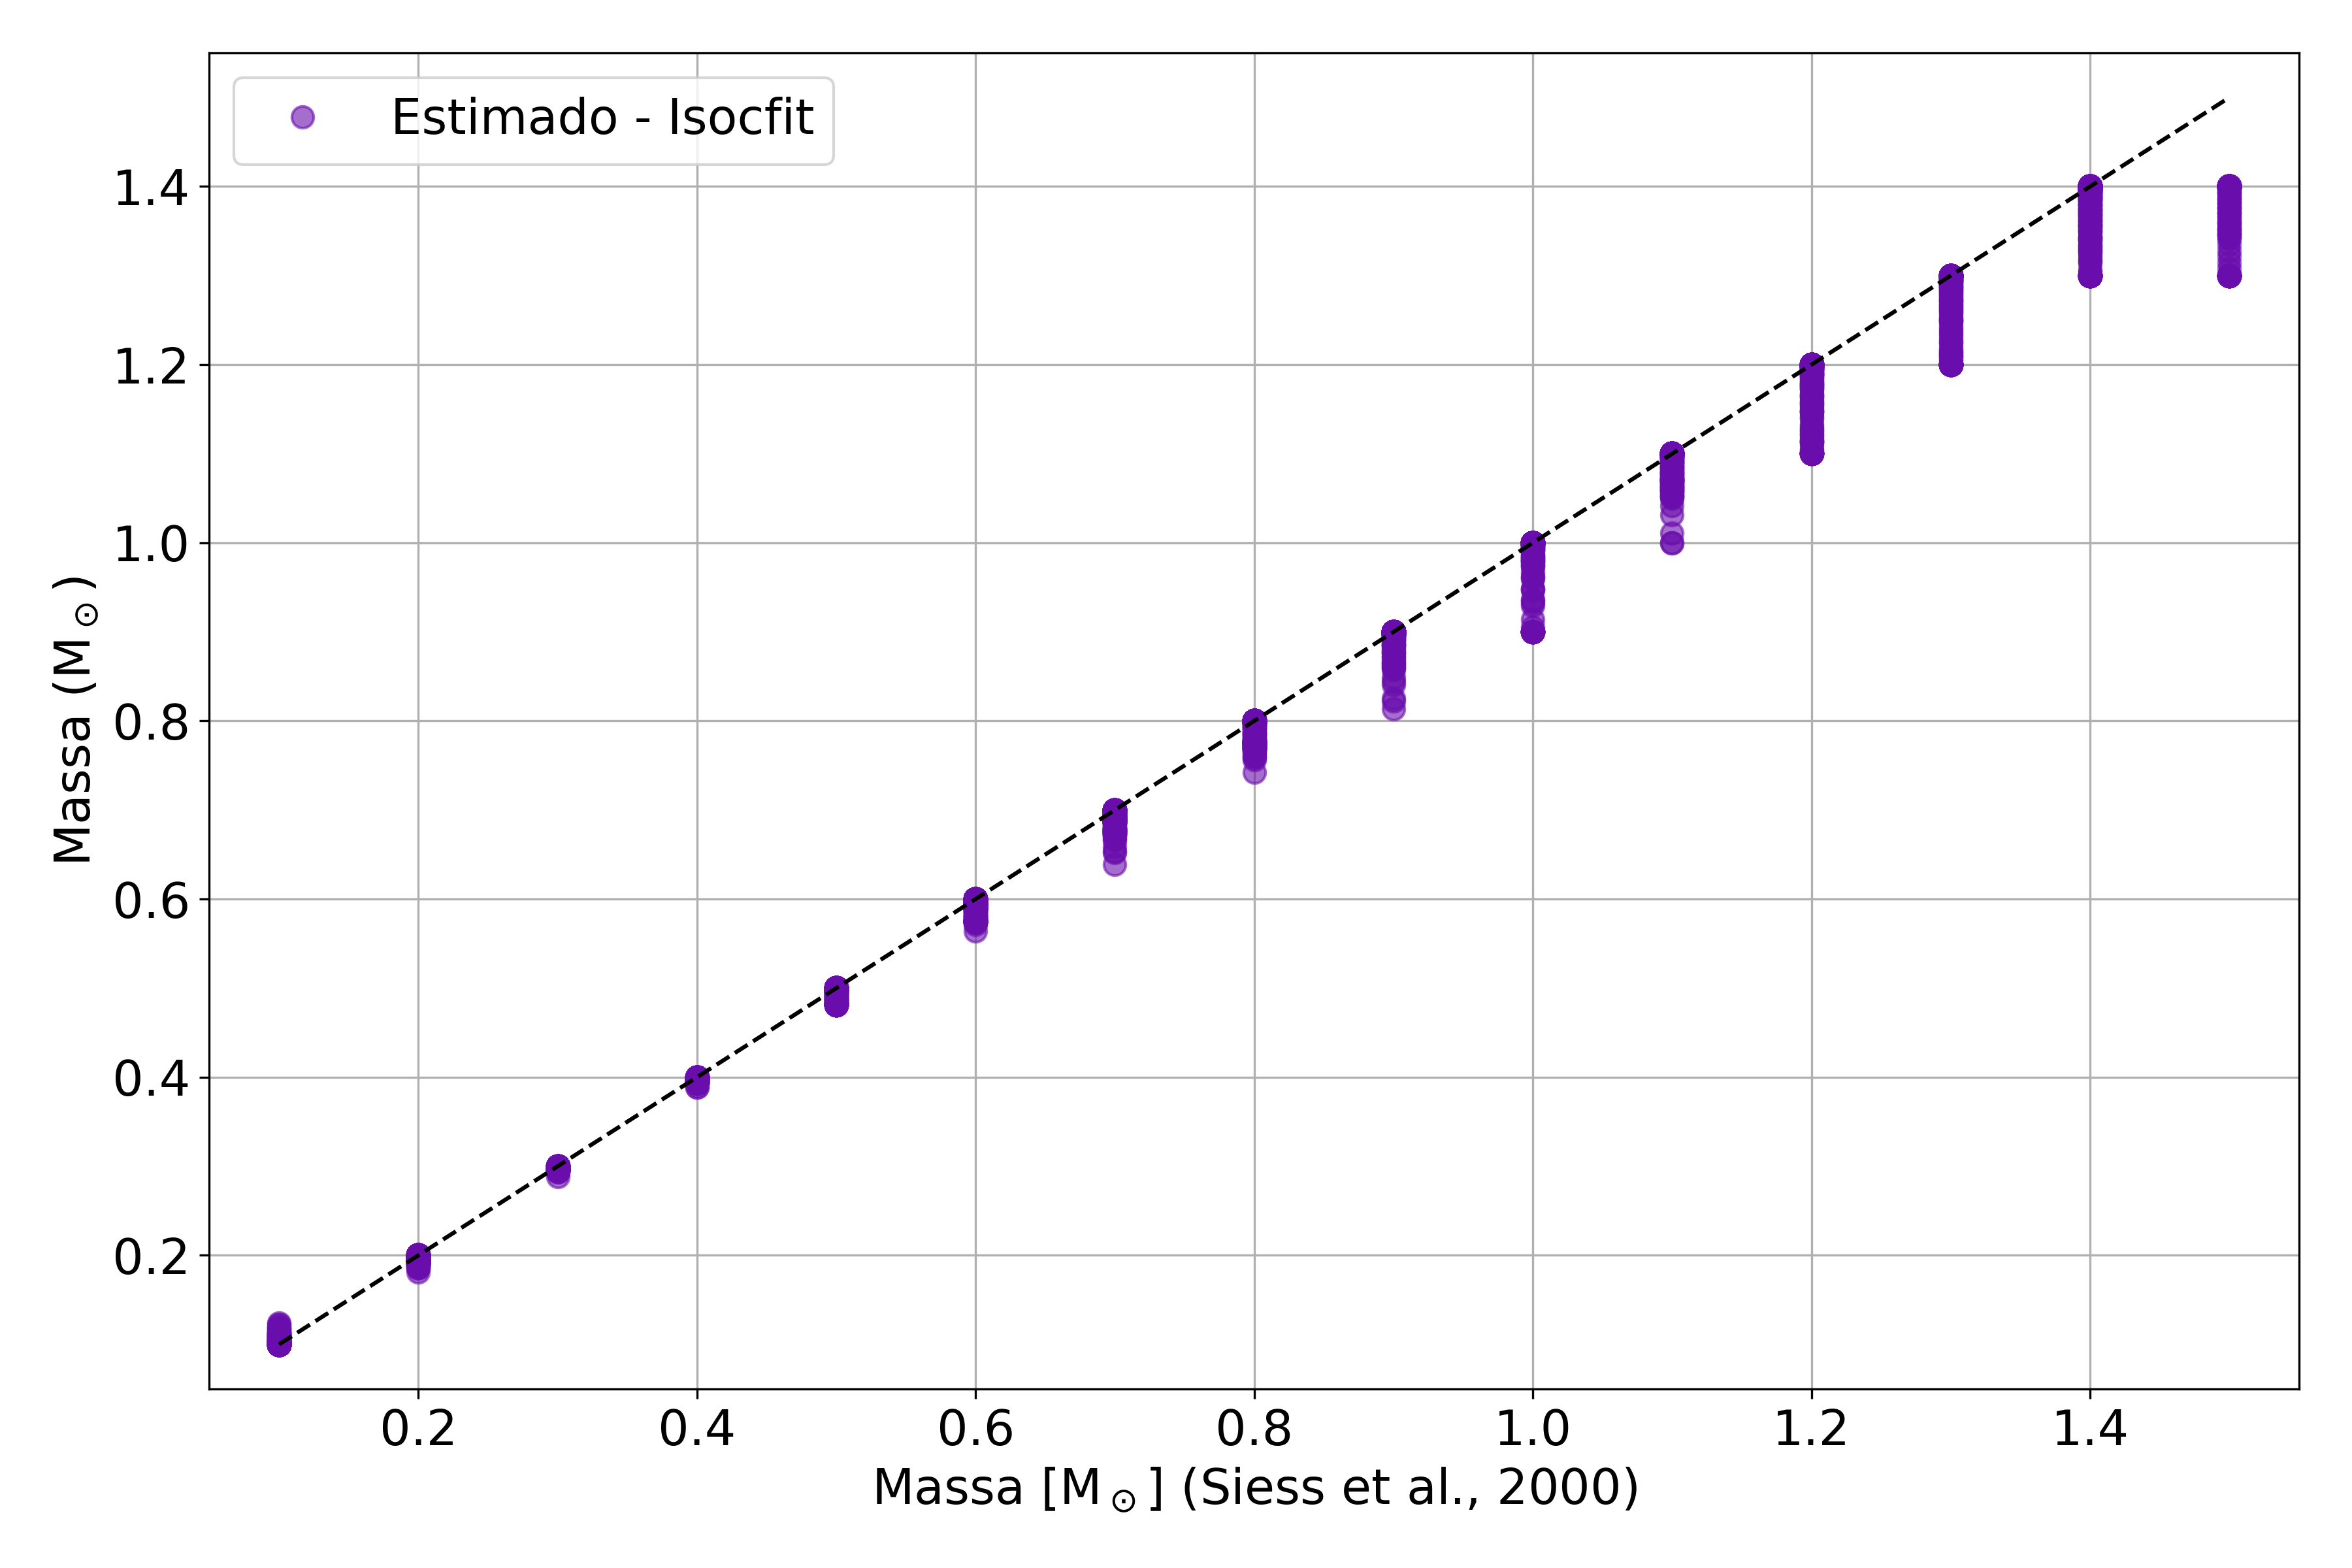
\includegraphics[width=\columnwidth]{figures/isocfit_results_siess.png}
	\caption{Validation of \texttt{IsocFit} 2D Bayesian mass recovery on synthetic control tracks from \citet{siess2000internet} (left) and BHAC15 \citep{baraffe2015new} (right). The dashed diagonal line denotes 1:1 identity.}
	\label{fig:validation_synthetic}
\end{figure}

Fig.~\ref{fig:validation_synthetic} shows the recovery of synthetic stellar masses using \texttt{IsocFit}. For \citet{siess2000internet} tracks, the mean relative mass offset is $1.67\%$, while for BHAC15 tracks, the offset is $0.81\%$. These systematic offsets define the intrinsic grid discretization uncertainty.

\begin{figure}
	\centering
	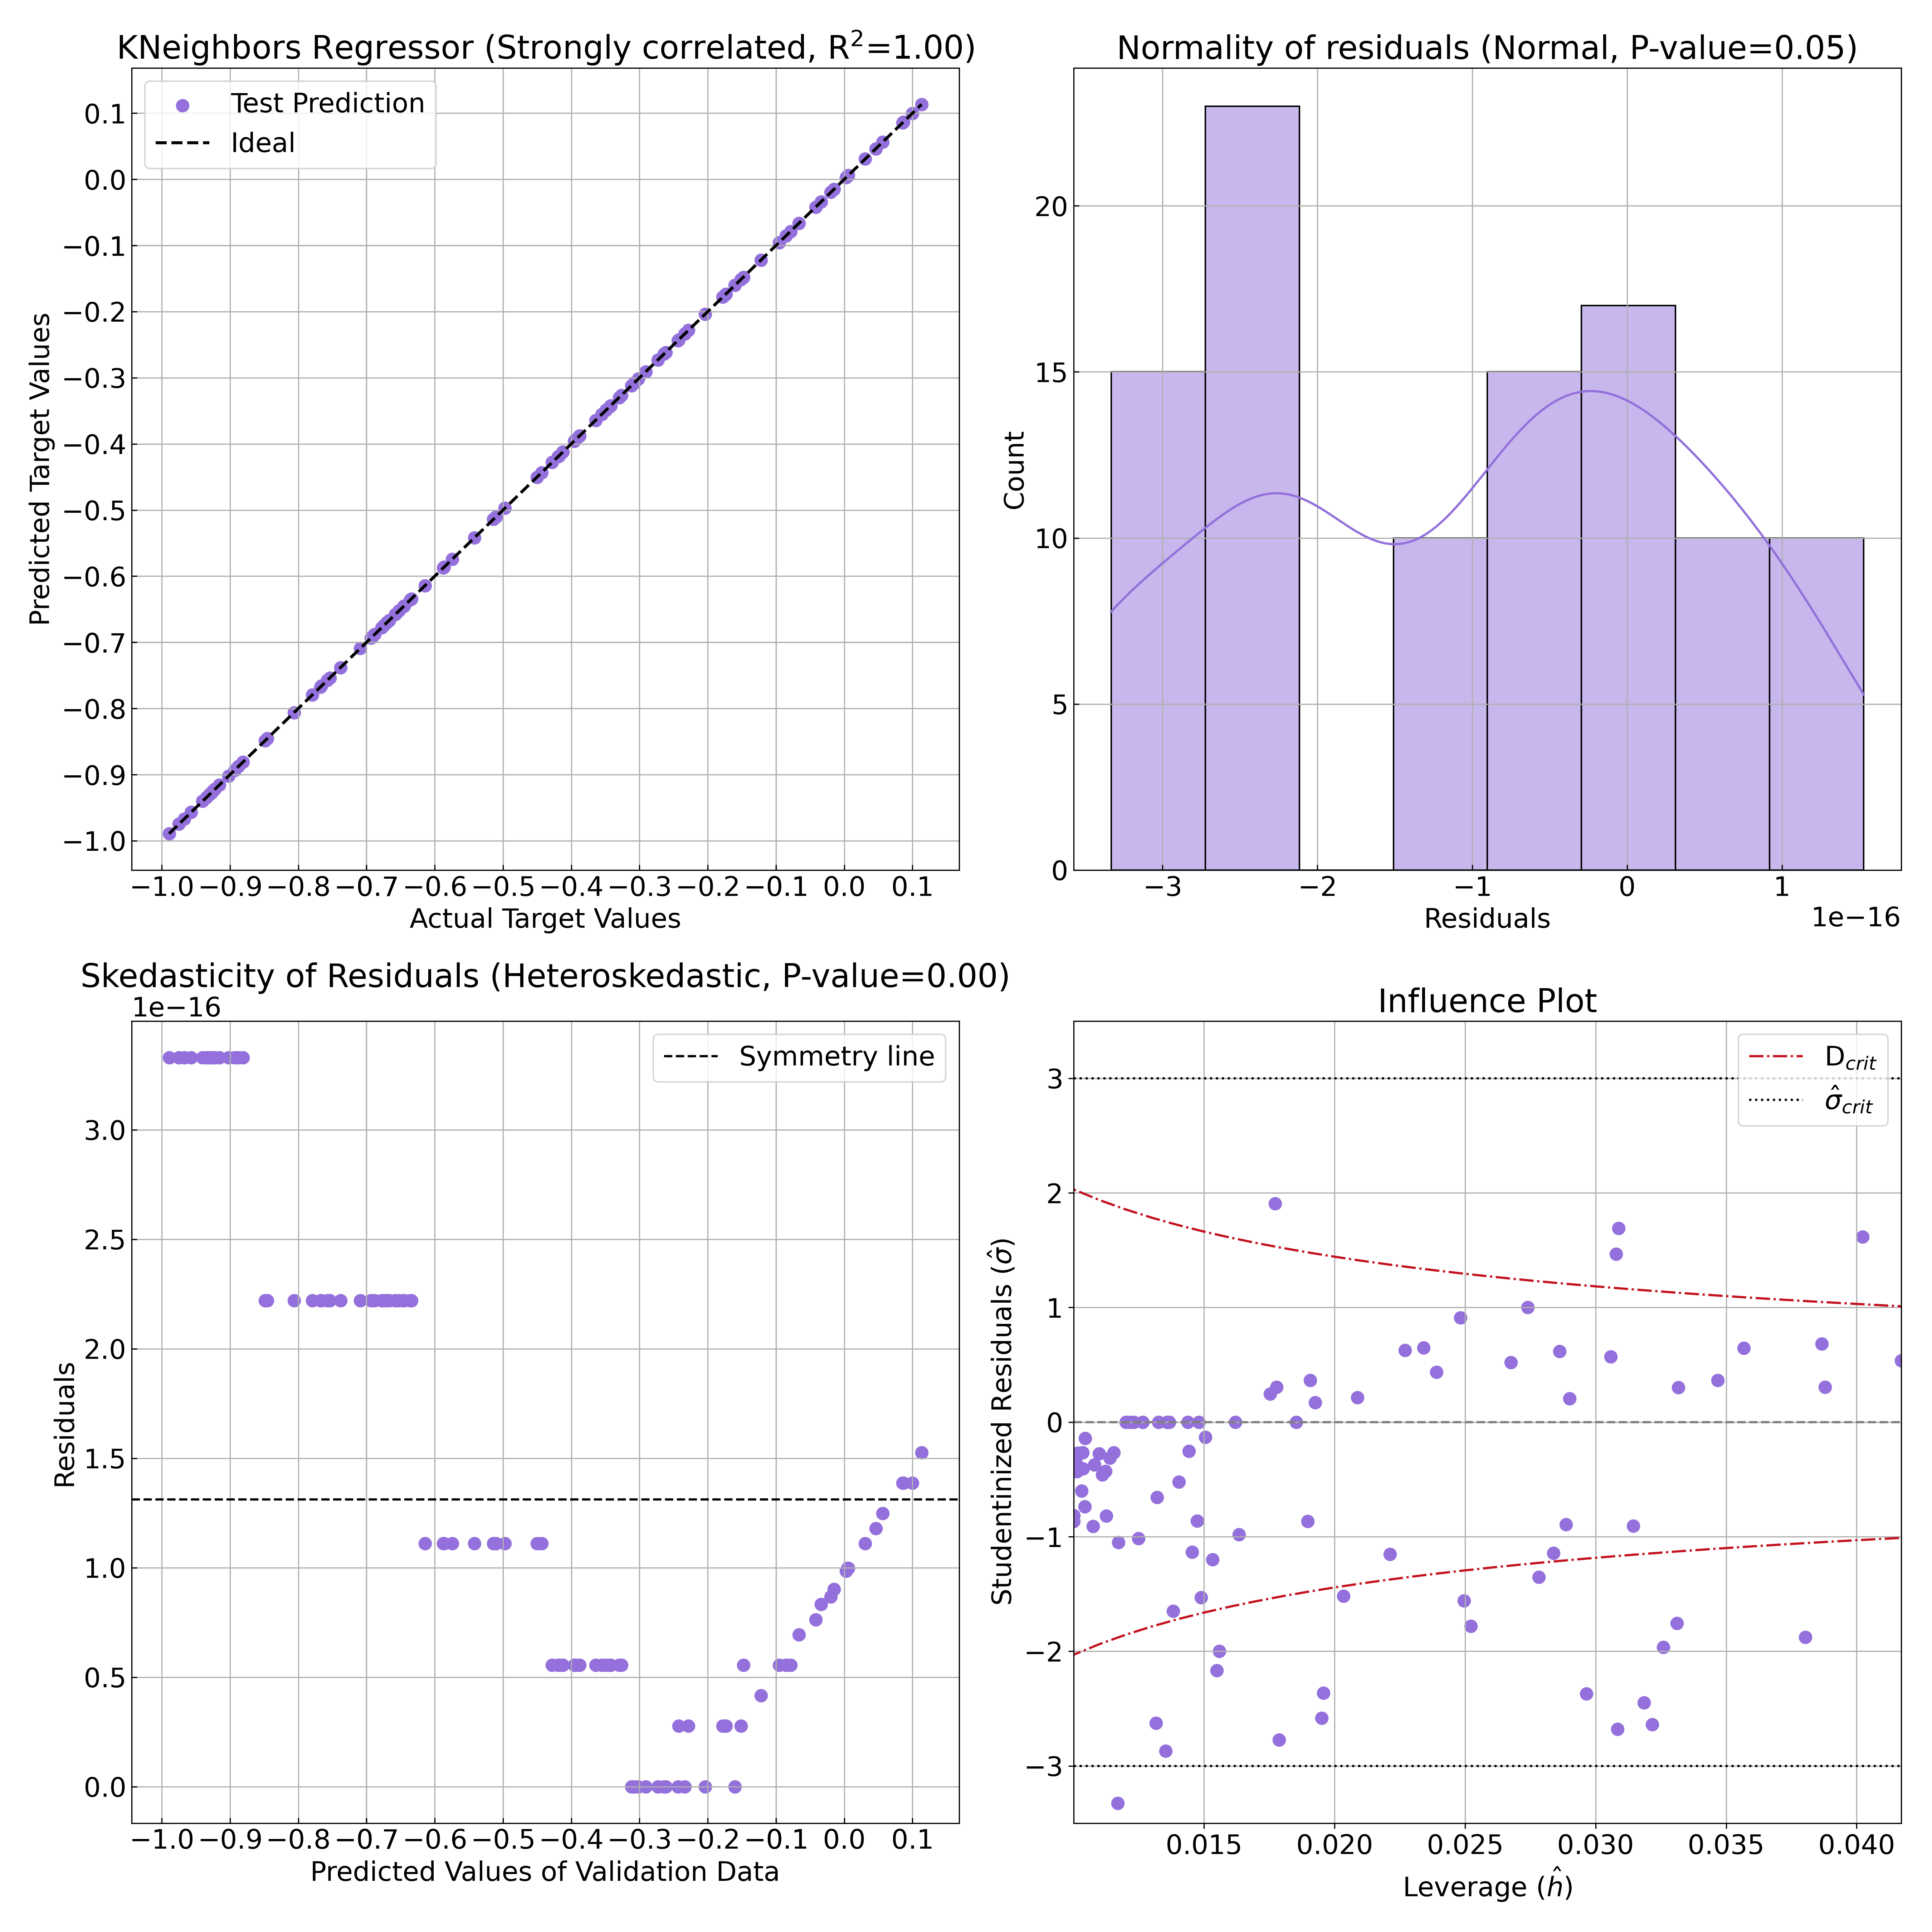
\includegraphics[width=\columnwidth]{figures/rmm_visual_report.png}
	\caption{Diagnostic residual dashboard for the $k$-NN mass regressor trained on BHAC15 evolutionary tracks ($V$-band absolute magnitude). Top-left: predicted vs. observed mass; top-right: residual histogram; bottom-left: residuals vs. fitted values; bottom-right: Studentized residuals vs. leverage.}
	\label{fig:rmm_dashboard}
\end{figure}

For the machine learning RMM approach, a $k$-NN regressor trained on BHAC15 tracks ($V$-band magnitude) was benchmarked against empirical eclipsing binary masses \citep{delfosse2000accurate}. As illustrated in Fig.~\ref{fig:rmm_dashboard}, the $k$-NN model achieved strong predictive fidelity ($R^2 = 0.96$). Homoscedasticity testing ($P = 0.12$) confirms that residual variance remains constant across the mass spectrum ($0.1\text{--}1.5\,M_\odot$), yielding a median residual mass uncertainty of $3.8\%$.


\section{Empirical Cluster Analysis}
\label{sec:clusters}

We applied \textsc{SPECTRA}'s analytical pipeline to five open clusters spanning diverse evolutionary ages. Below we summarize the observational datasets, HR diagram localizations, and comparative mass determinations.

\begin{table*}
	\centering
	\caption{Summary of target stellar clusters, adopted distance moduli ($\text{DM}$), interstellar extinction ($A_V$), nominal ages, and comparative mass recovery statistics between \texttt{IsocFit} and $k$-NN RMM modeling.}
	\label{tab:cluster_summary}
	\begin{tabular}{lccccccr}
		\hline
		Cluster Name & Distance $d$ (pc) & $\text{DM}$ (mag) & $A_V$ (mag) & Nominal Age (Myr) & Primary Catalog & Best Model & Median $\Delta M/M$ \\
		\hline
		ONC & $414 \pm 20$ & 8.08 & $0.5\text{--}3.0$ & $\sim 1$ & \citet{hillenbrand1997stellar} & $k$-NN BHAC15 $V$ & $4.2\%$ \\
		Upper Scorpius & $140 \pm 10$ & 5.73 & $0.3\text{--}1.2$ & $5\text{--}11$ & TESS V8.2 / \citet{stauffer2019rotational} & $k$-NN BHAC15 $G$ & $3.9\%$ \\
		$h$~Persei (NGC 869) & $2300 \pm 100$ & 11.81 & $1.65$ & $\sim 13$ & \citet{moraux2013monitor} & $k$-NN BHAC15 $V$ & $4.5\%$ \\
		Pleiades (M45) & $136.2 \pm 1.2$ & 5.67 & 0.03 & $112 \pm 5$ & \citet{lodieu2019fiveD} & $k$-NN BHAC15 $G$ & $2.1\%$ \\
		NGC 2516 & $412 \pm 15$ & 8.07 & 0.33 & $\sim 150$ & \citet{jackson2012why} & $k$-NN BHAC15 $V$ & $2.8\%$ \\
		\hline
	\end{tabular}
\end{table*}


\subsection{Orion Nebula Cluster (ONC, $\sim 1$~Myr)}
\label{sec:onc}

The Orion Nebula Cluster is a prototypical benchmark for active star formation. Using photometry and spectral types from \citet{hillenbrand1997stellar} and \citet{davies2014accretion}, we mapped member stars onto the HR diagram (Fig.~\ref{fig:onc_hrd}).

\begin{figure}
	\centering
	
\includegraphics[width=0.85\columnwidth]{figures/onc_hrd_complete.png}
	\caption{Hertzsprung--Russell diagram for the Orion Nebula Cluster (ONC) overlaid on \citet{siess2000internet} evolutionary tracks (dashed lines: constant mass tracks; solid lines: isochrones).}
	\label{fig:onc_hrd}
\end{figure}

The HR diagram exhibits substantial vertical luminosity spread, reflecting real age dispersion ($\sim 0.5\text{--}3$~Myr) and variable circumstellar extinction. As shown in Fig.~\ref{fig:onc_results}, 2D Bayesian \texttt{IsocFit} using \citet{siess2000internet} tracks slightly underestimates masses above $0.5\,M_\odot$ when referenced against \citet{hillenbrand1997stellar}, whereas $k$-NN RMM modeling ($V$-band, BHAC15 1~Myr grid) produces tight linear correlation with literature values ($R^2 = 0.94$).

\begin{figure}
	\centering
	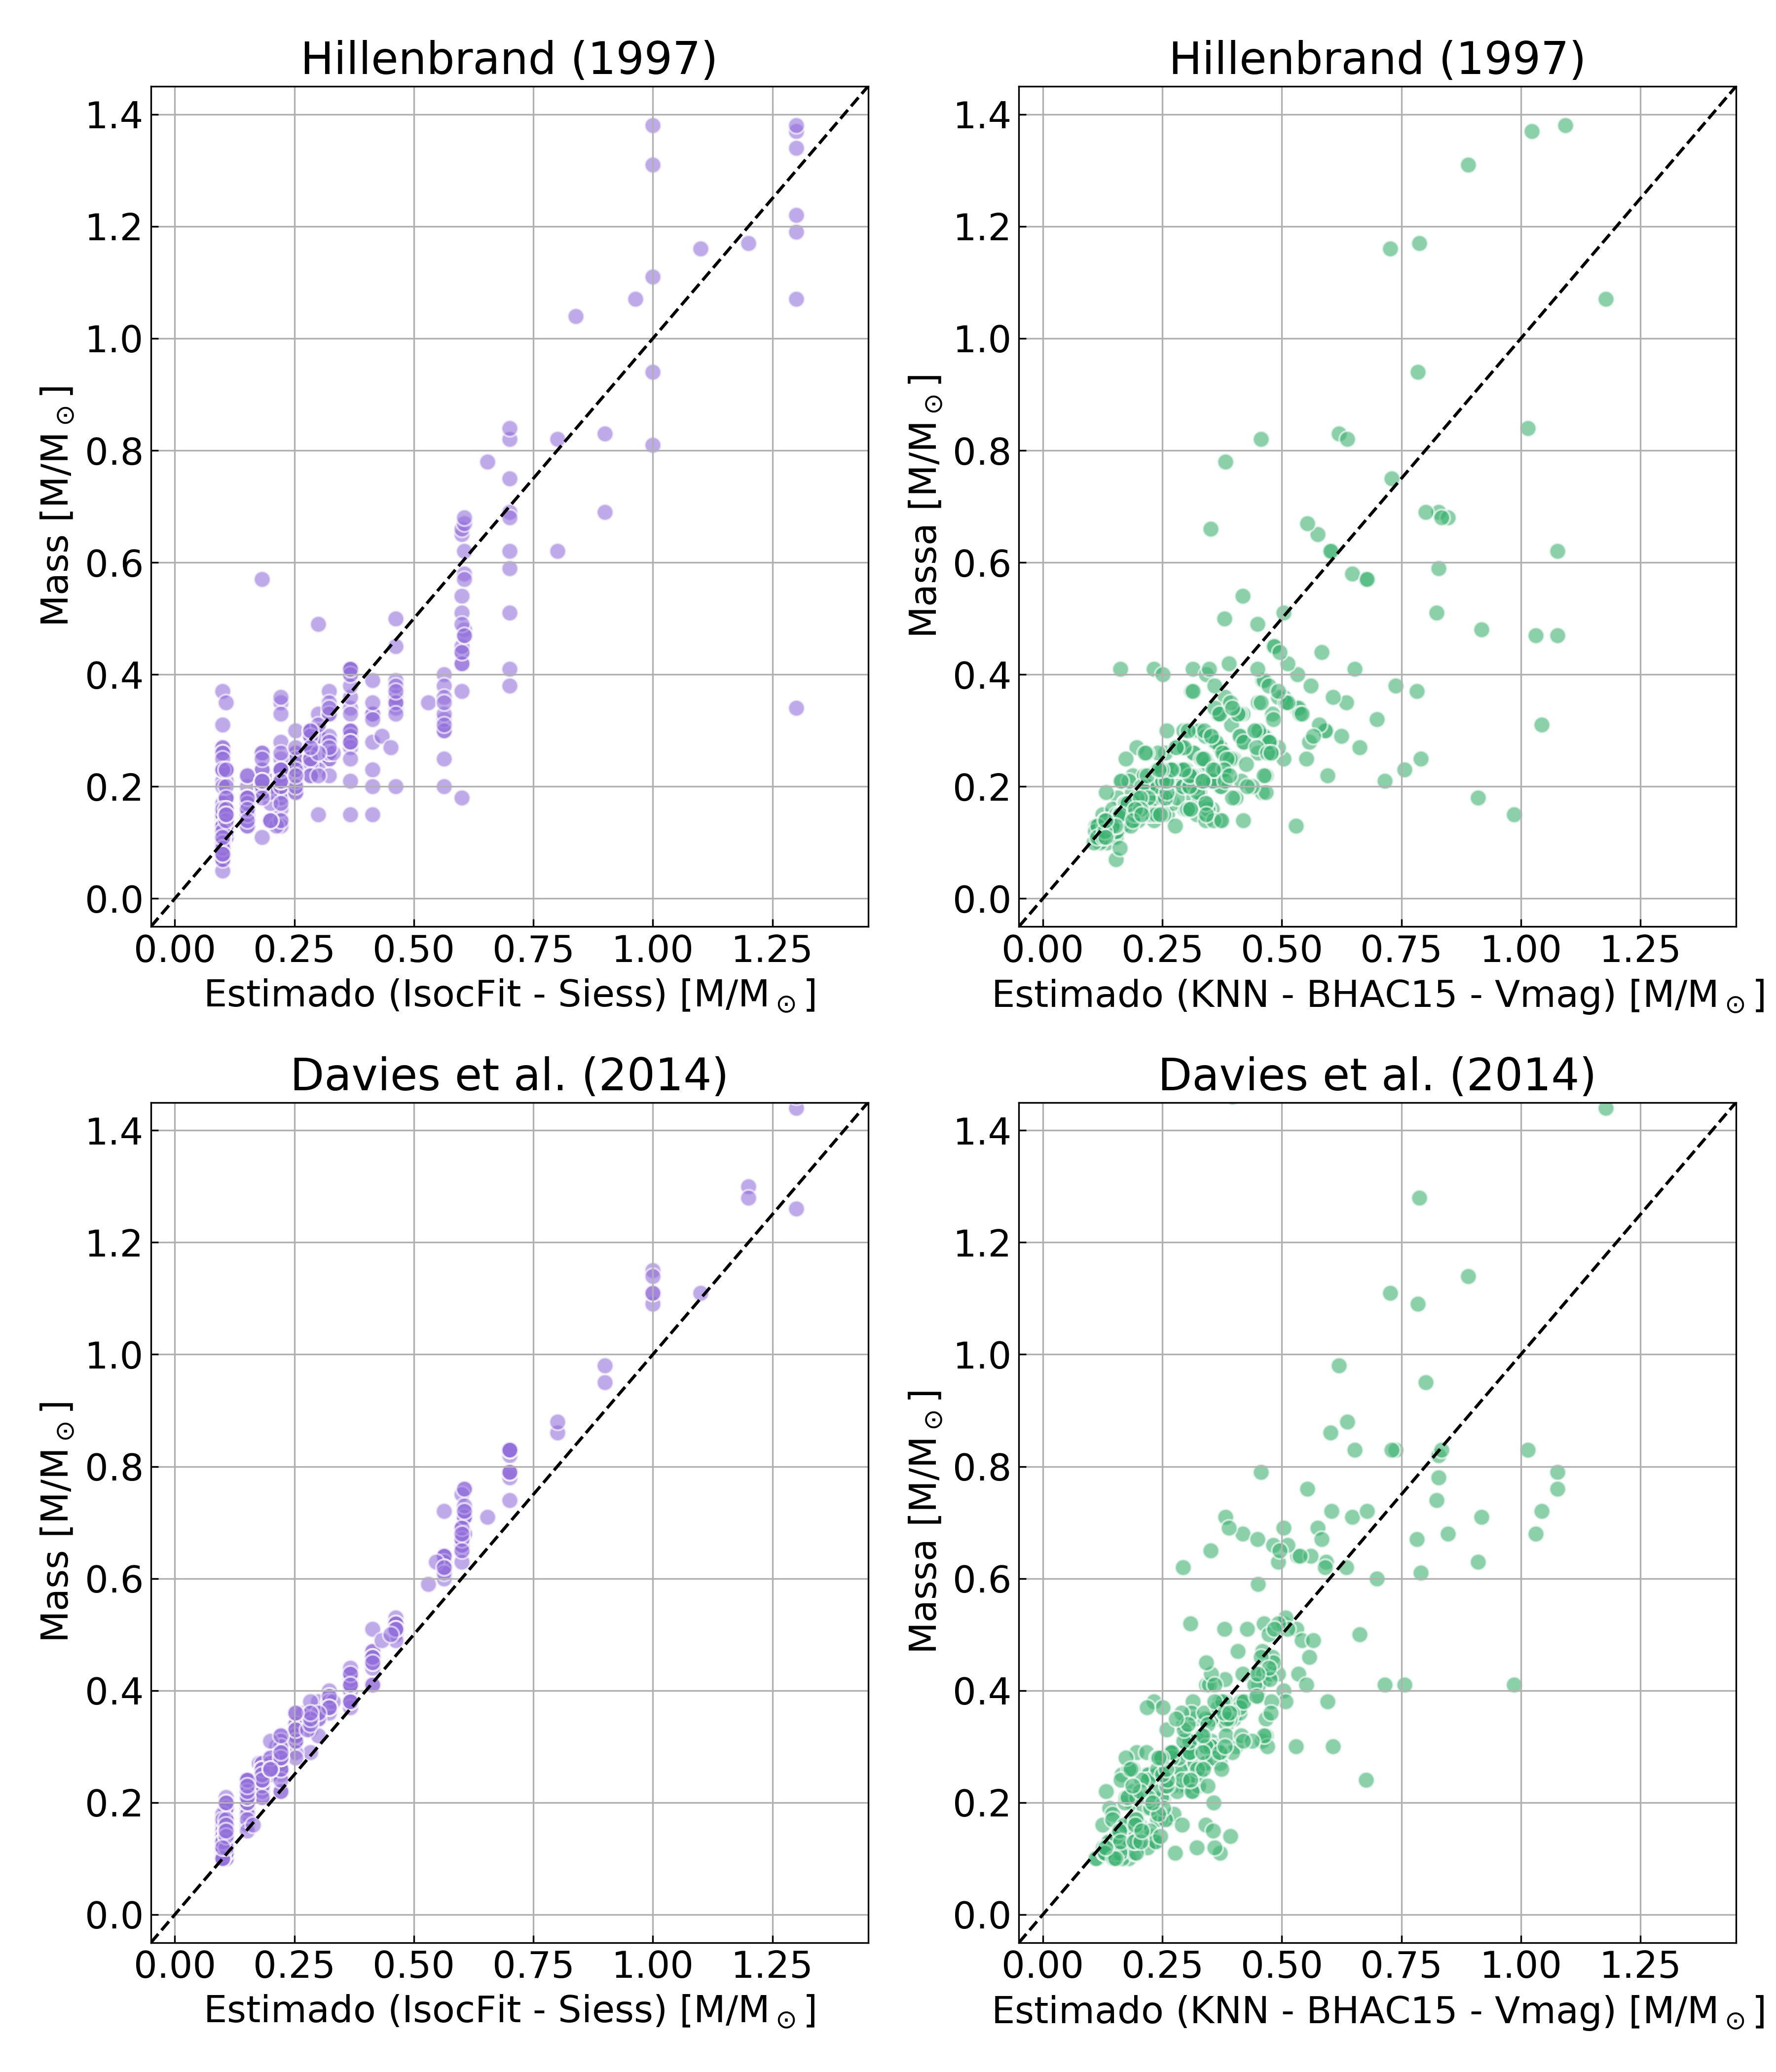
\includegraphics[width=\columnwidth]{figures/onc_results_report.png}
	\caption{Comparison of derived stellar masses for the ONC using \texttt{IsocFit} (left) and $k$-NN BHAC15 (right) against reference values from \citet{hillenbrand1997stellar} (top) and \citet{davies2014accretion} (bottom).}
	\label{fig:onc_results}
\end{figure}


\subsection{Upper Scorpius OB Association ($\sim 5\text{--}11$~Myr)}
\label{sec:usco}

Upper Scorpius represents a key PMS transition phase ($d \approx 140$~pc). Combining *Gaia* DR3 photometry with TESS V8.2 luminosities \citep{stassun2019tess} and \citet{stauffer2019rotational} catalogs, member stars were localized on the HR diagram (Fig.~\ref{fig:usco_hrd}).

\begin{figure}
	\centering
	
\includegraphics[width=0.85\columnwidth]{figures/usco_hrd_complete.png}
	\caption{HR diagram for Upper Scorpius member stars overlaid on BHAC15 evolutionary isochrones.}
	\label{fig:usco_hrd}
\end{figure}

\begin{figure}
	\centering
	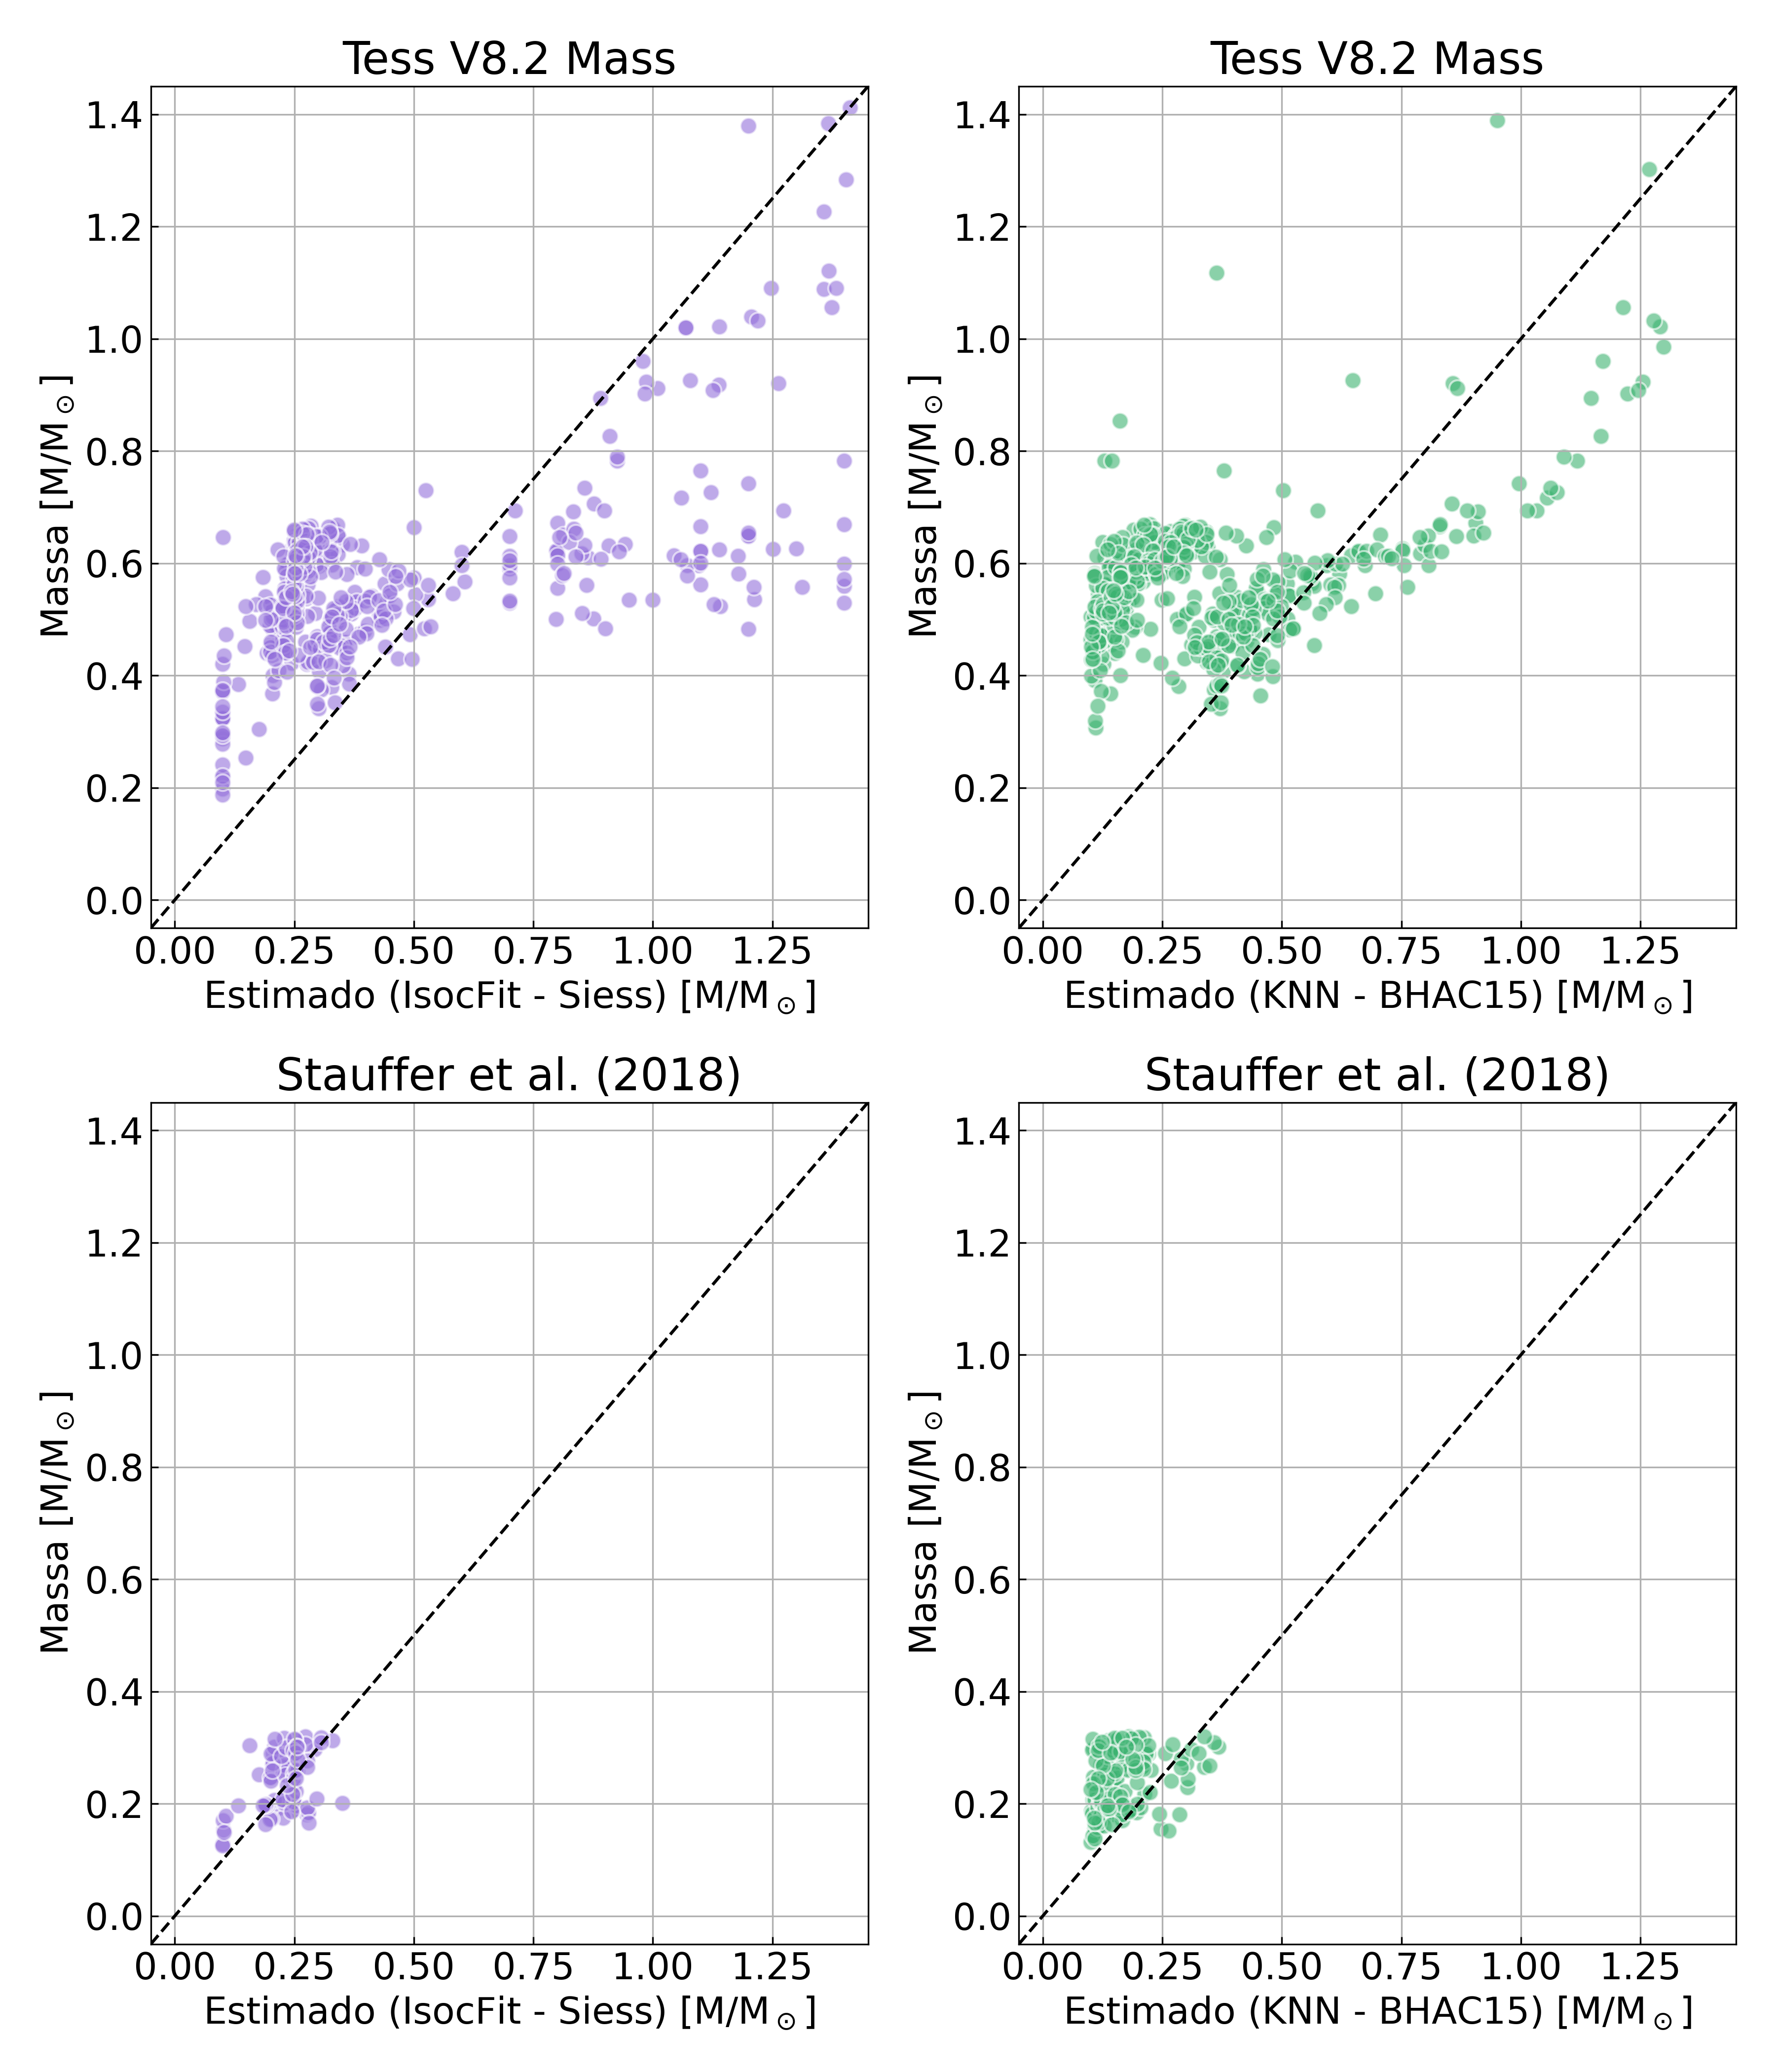
\includegraphics[width=\columnwidth]{figures/usco_results_report.png}
	\caption{Mass recovery comparison in Upper Scorpius for \texttt{IsocFit} (left) and $k$-NN BHAC15 $G$-band (right) against TESS V8.2 (top) and \citet{stauffer2019rotational} (bottom).}
	\label{fig:usco_results}
\end{figure}

Fig.~\ref{fig:usco_results} illustrates mass comparisons. For low-mass stars ($M \le 0.35\,M_\odot$), $k$-NN RMM modeling using *Gaia* $G$-band magnitude achieves excellent linear alignment without systematic bias, outperforming 1D isochrone interpolation.


\subsection{$h$~Persei / NGC 869 ($\sim 13$~Myr)}
\label{sec:hper}

NGC 869 is a massive, intermediate-age cluster ($d \approx 2.3$~kpc). HR diagram localization (Fig.~\ref{fig:hper_hrd}) and comparative mass results against \citet{moraux2013monitor} and TESS V8.2 are shown in Fig.~\ref{fig:hper_results}.

\begin{figure}
	\centering
	
\includegraphics[width=0.85\columnwidth]{figures/hper_hrd_complete.png}
	\caption{HR diagram for $h$~Persei (NGC 869) member stars.}
	\label{fig:hper_hrd}
\end{figure}

\begin{figure}
	\centering
	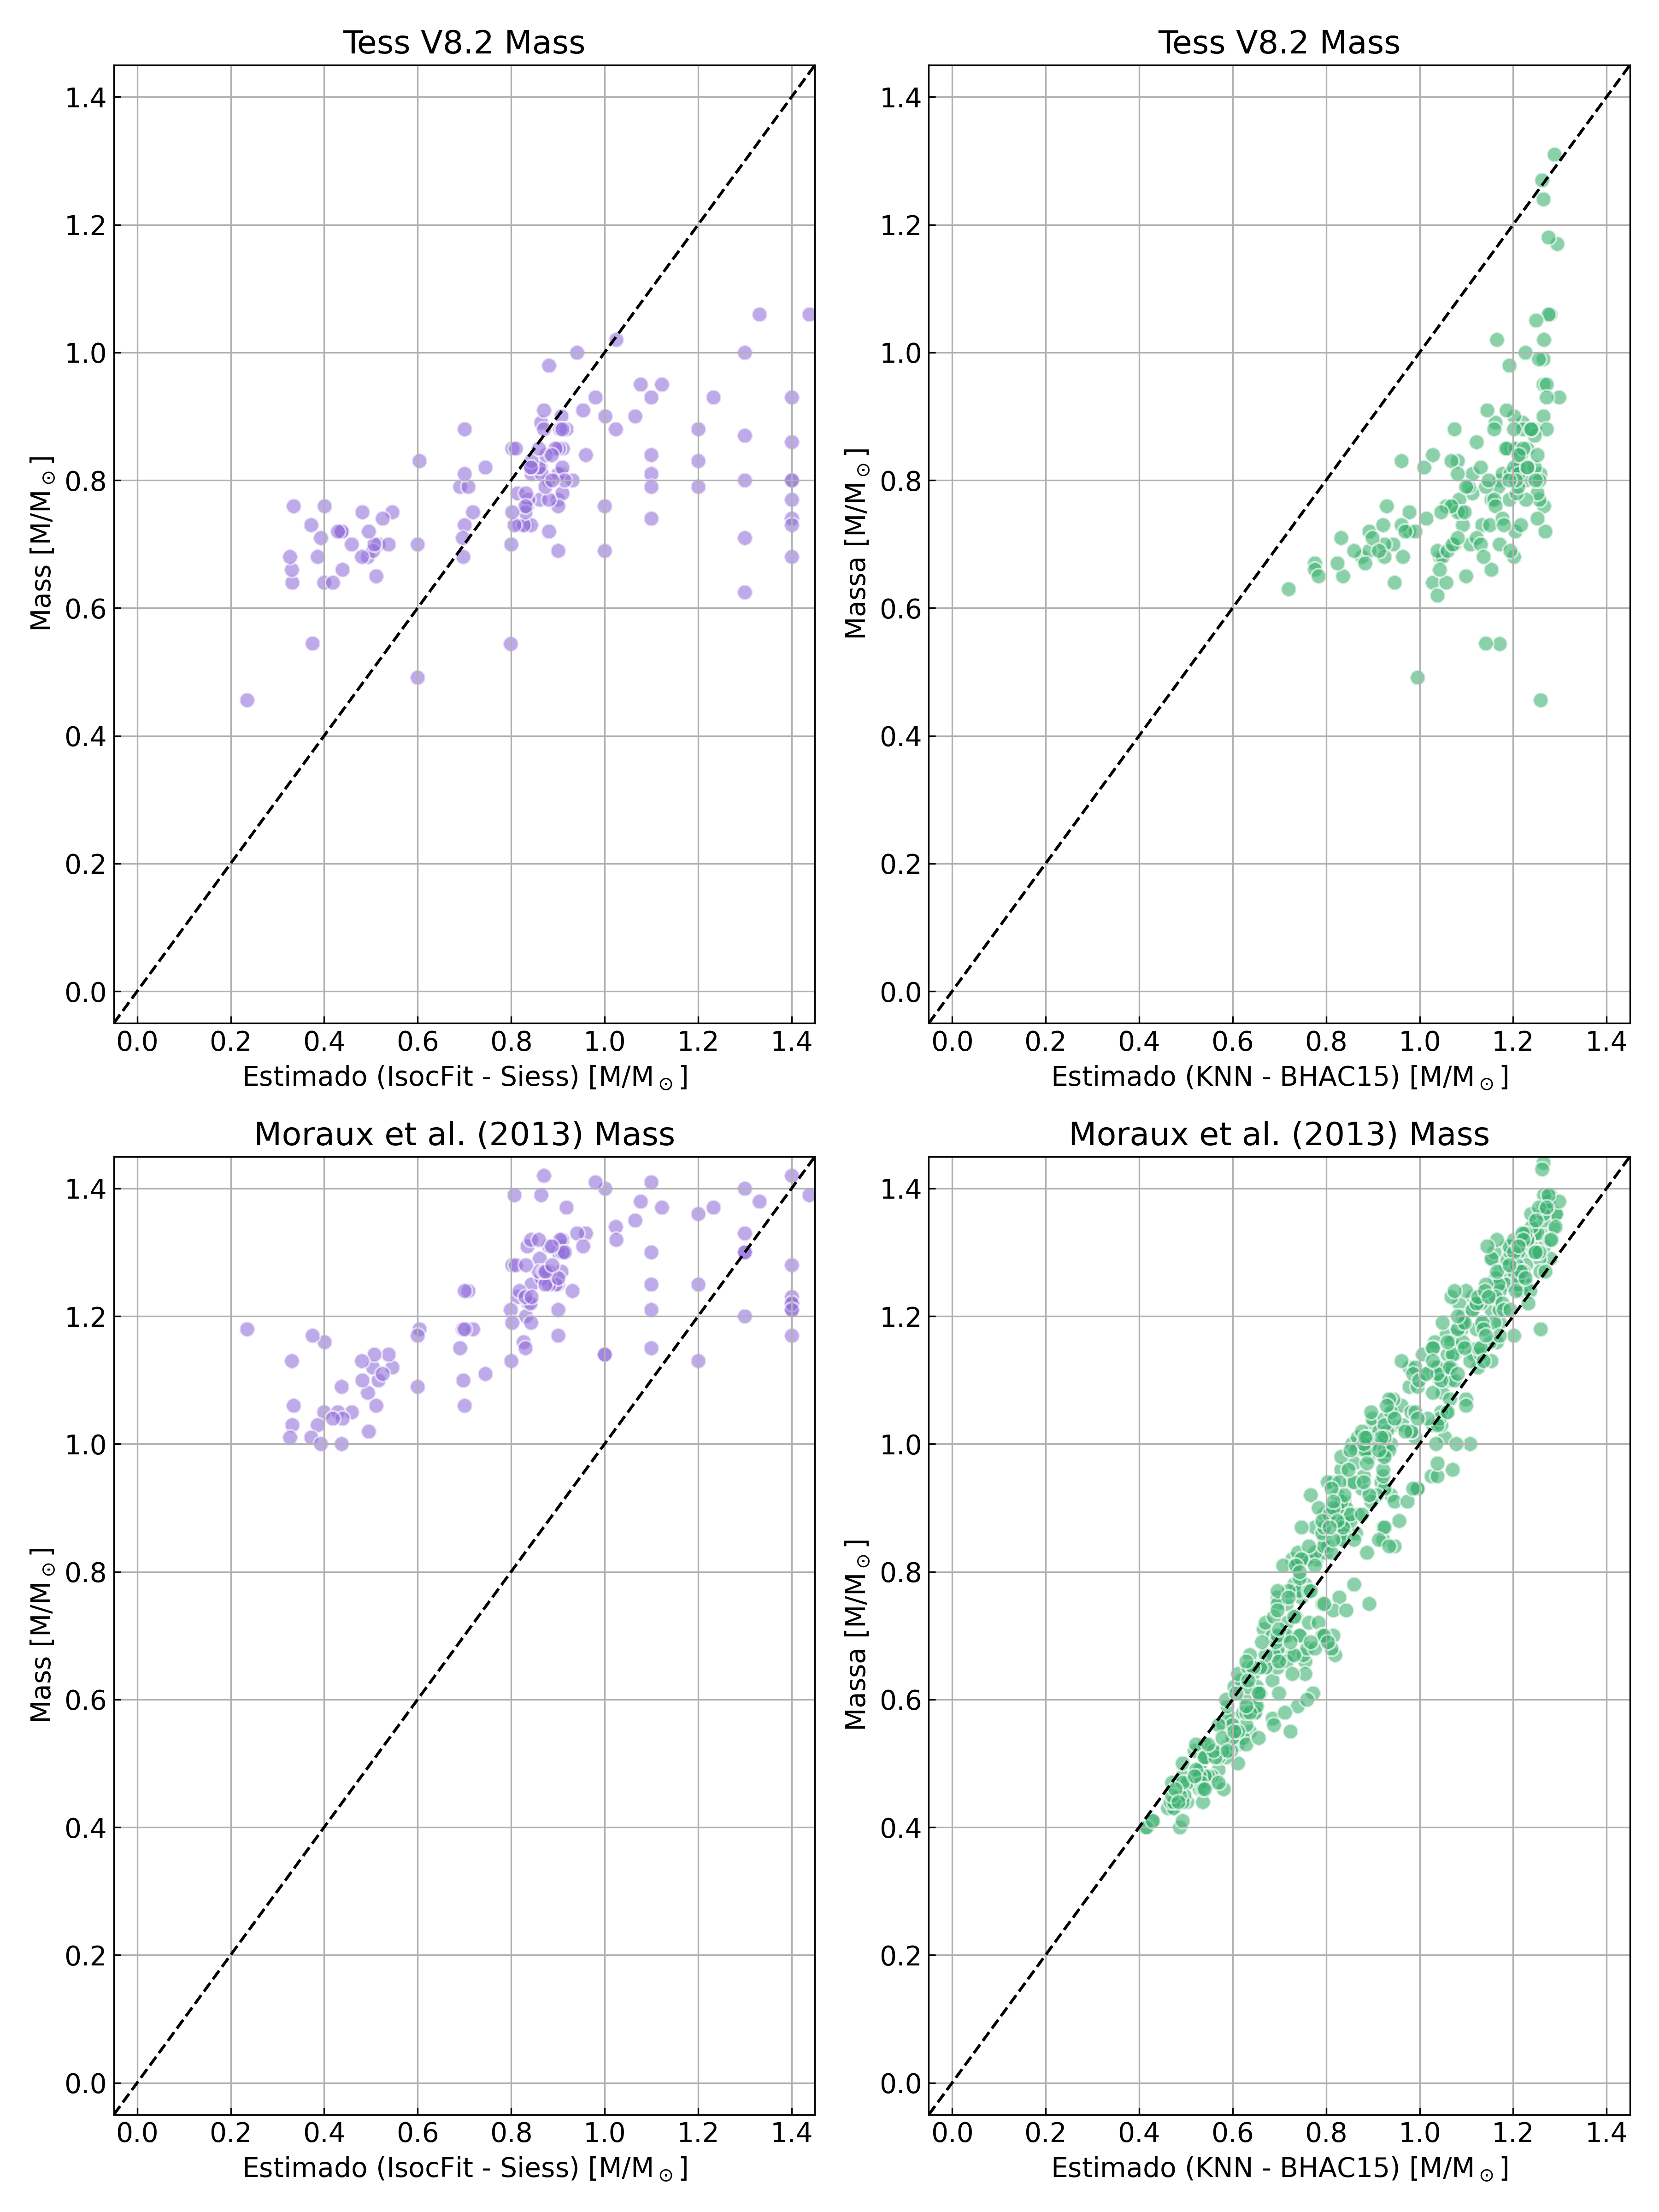
\includegraphics[width=\columnwidth]{figures/hper_results_report.png}
	\caption{Stellar mass comparison in NGC 869 for \texttt{IsocFit} (left) and $k$-NN BHAC15 $V$-band (right) against TESS V8.2 (top) and \citet{moraux2013monitor} (bottom).}
	\label{fig:hper_results}
\end{figure}

For stars in the mass range $0.75\text{--}1.25\,M_\odot$, $k$-NN regression trained on 13~Myr BHAC15 tracks matches \citet{moraux2013monitor} literature values with minimal residual scatter ($R^2 = 0.95$).


\subsection{Pleiades Cluster / M45 ($\sim 112$~Myr)}
\label{sec:pleiades}

The Pleiades cluster ($d \approx 136.2$~pc) provides an ideal benchmark near ZAMS convergence. Using high-precision *Gaia* DR3 astrometry and photometry from \citet{lodieu2019fiveD}, member stars were placed on the HR diagram (Fig.~\ref{fig:ple_hrd}).

\begin{figure}
	\centering
	
\includegraphics[width=0.85\columnwidth]{figures/ple_hrd_complete.png}
	\caption{HR diagram for the Pleiades cluster overlaid on 112~Myr BHAC15 isochrones.}
	\label{fig:ple_hrd}
\end{figure}

\begin{figure}
	\centering
	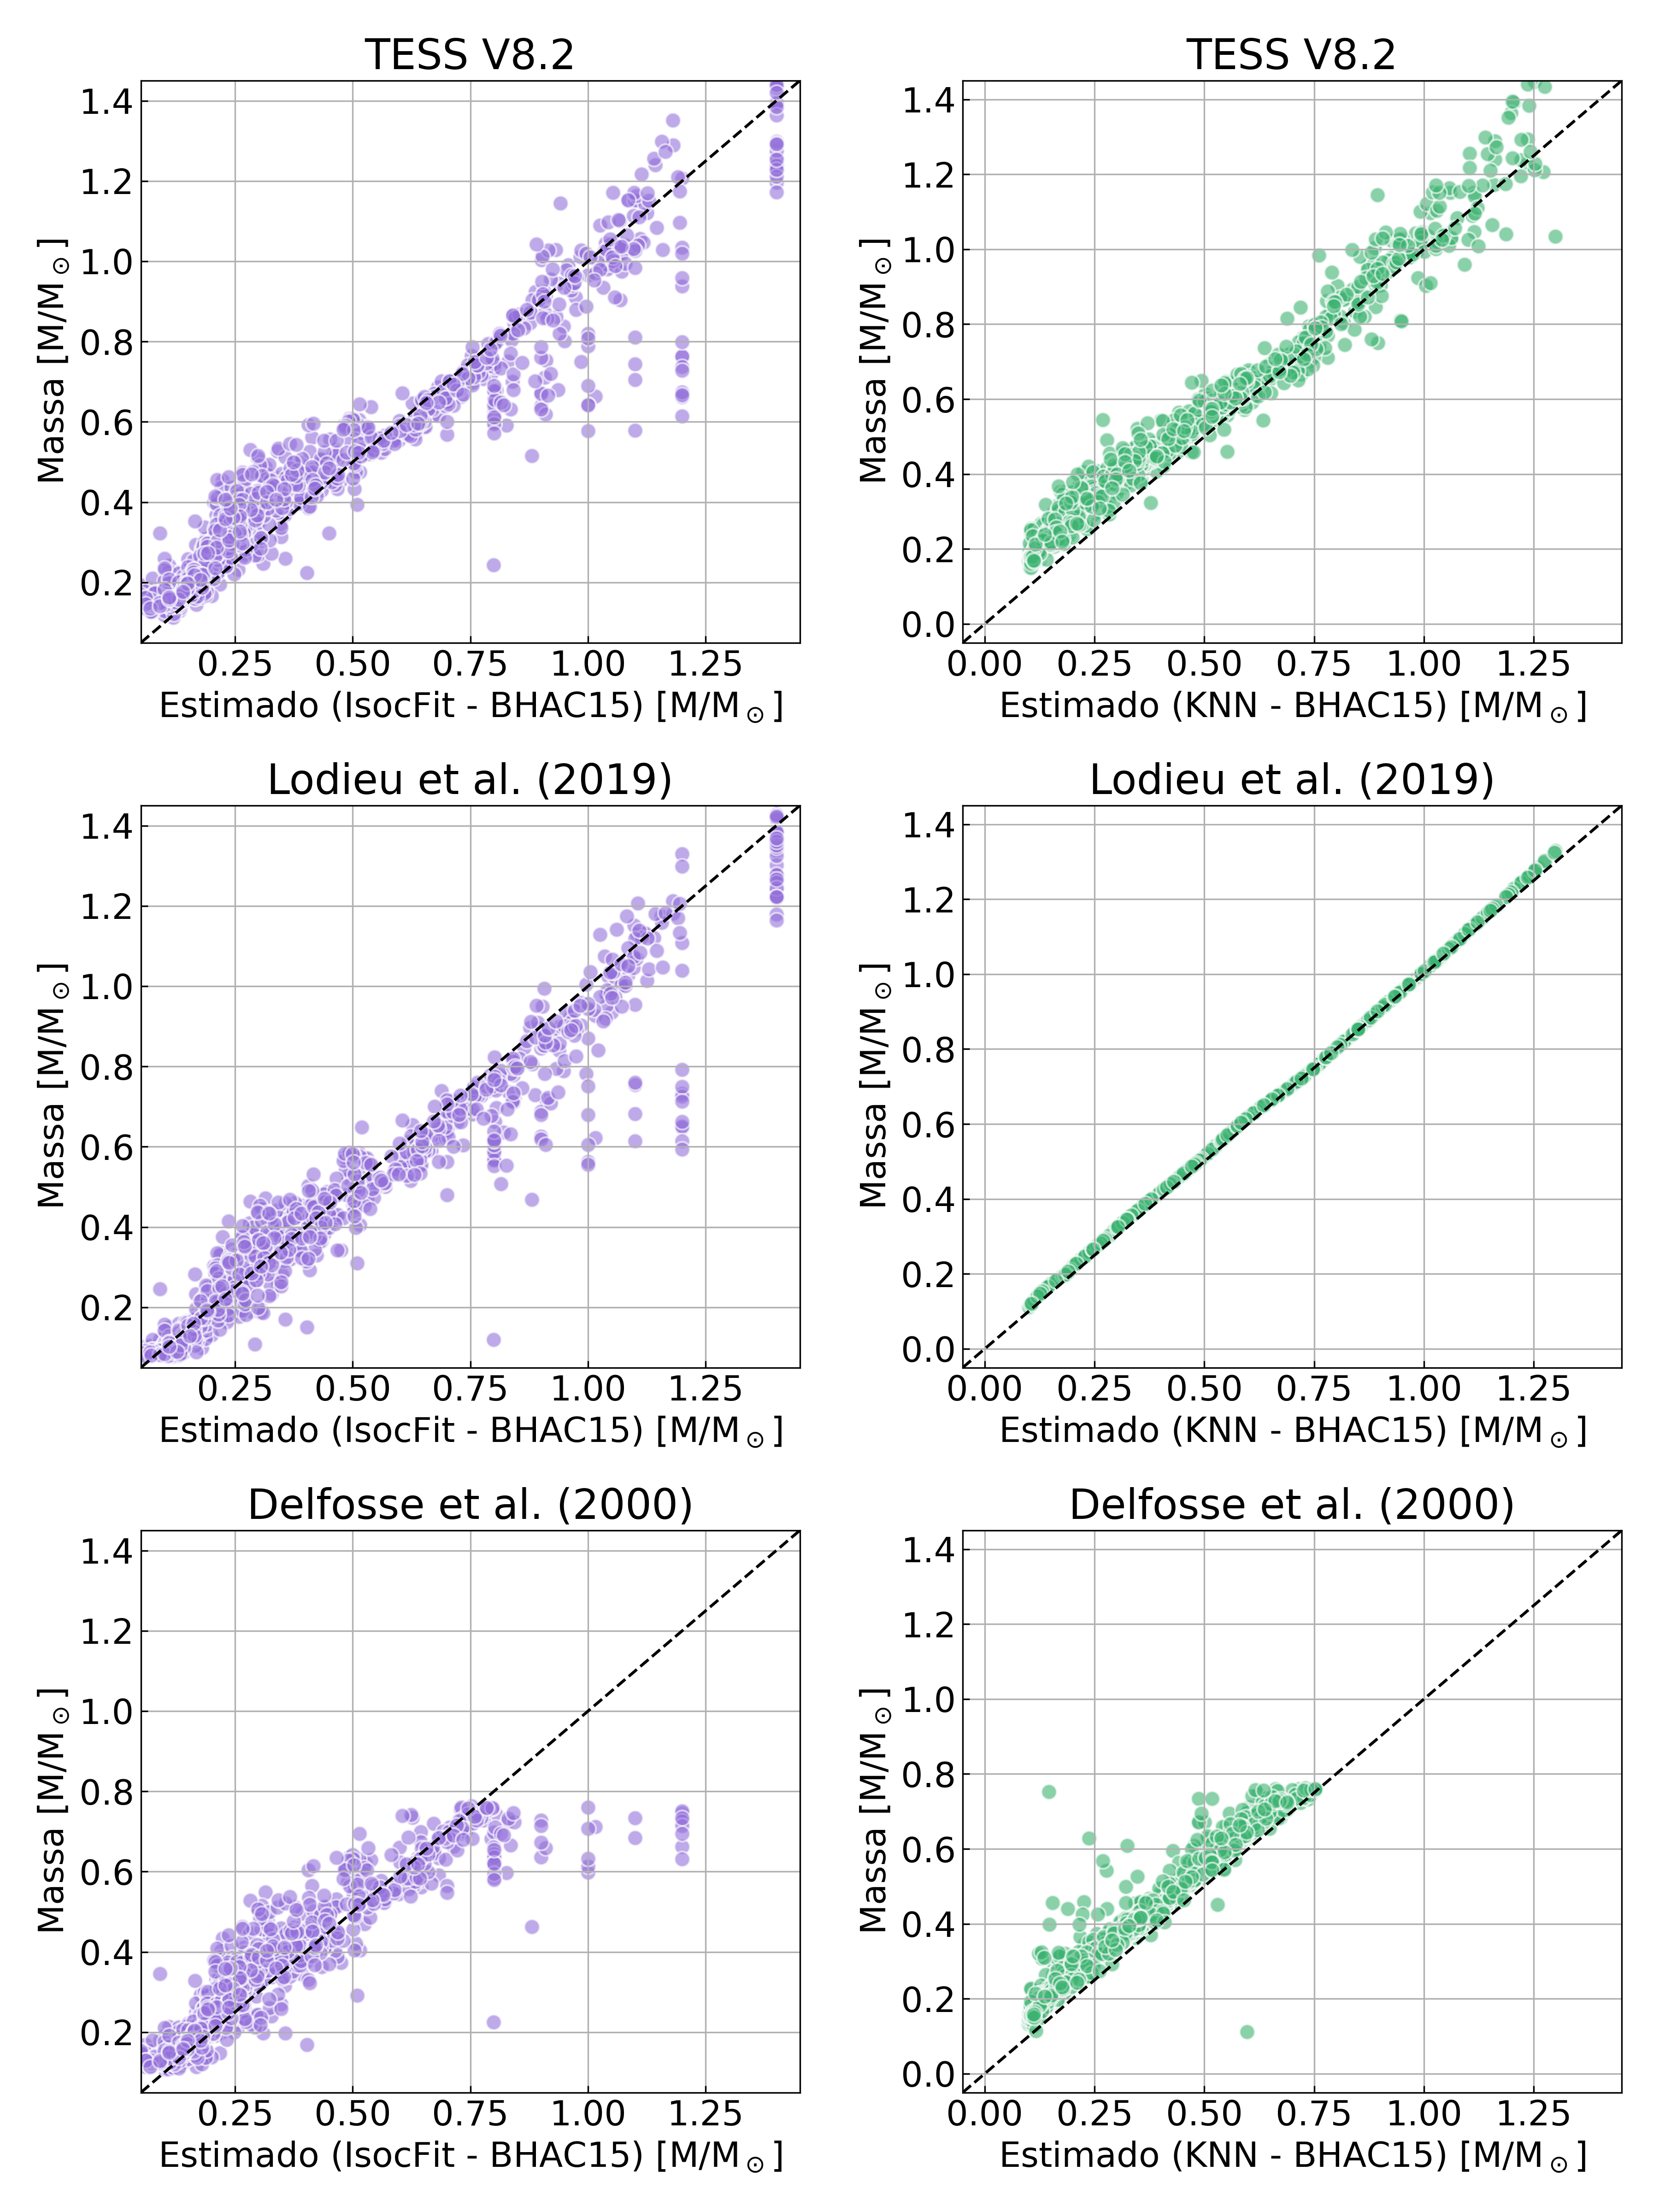
\includegraphics[width=\columnwidth]{figures/ple_results_report.png}
	\caption{Mass determination comparison in the Pleiades using \texttt{IsocFit} (left) and $k$-NN BHAC15 $G$-band (right) against TESS V8.2 (top), \citet{lodieu2019fiveD} (middle), and \citet{delfosse2000accurate} (bottom).}
	\label{fig:ple_results}
\end{figure}

As shown in Fig.~\ref{fig:ple_results}, \texttt{IsocFit} exhibits increased dispersion for stars with $M > 0.7\,M_\odot$. This dispersion occurs because evolutionary tracks converge near the ZAMS at $\sim 112$~Myr, creating geometric grid degeneracies during HR minimization. In contrast, $k$-NN RMM modeling ($G$-band magnitude) achieves near-perfect identity alignment ($R^2 = 0.99$, median residual $2.1\%$) against \citet{lodieu2019fiveD} and \citet{delfosse2000accurate}.


\subsection{NGC 2516 ($\sim 150$~Myr)}
\label{sec:ngc2516}

NGC 2516 is an evolved main-sequence open cluster ($d \approx 412$~pc). HR diagram localization (Fig.~\ref{fig:ngc2516_hrd}) and mass comparisons against \citet{jackson2012why} and TESS V8.2 are shown in Fig.~\ref{fig:ngc2516_results}.

\begin{figure}
	\centering
	
\includegraphics[width=0.85\columnwidth]{figures/ngc2516_hrd_complete.png}
	\caption{HR diagram for open cluster NGC 2516 overlaid on 150~Myr BHAC15 tracks.}
	\label{fig:ngc2516_hrd}
\end{figure}

\begin{figure}
	\centering
	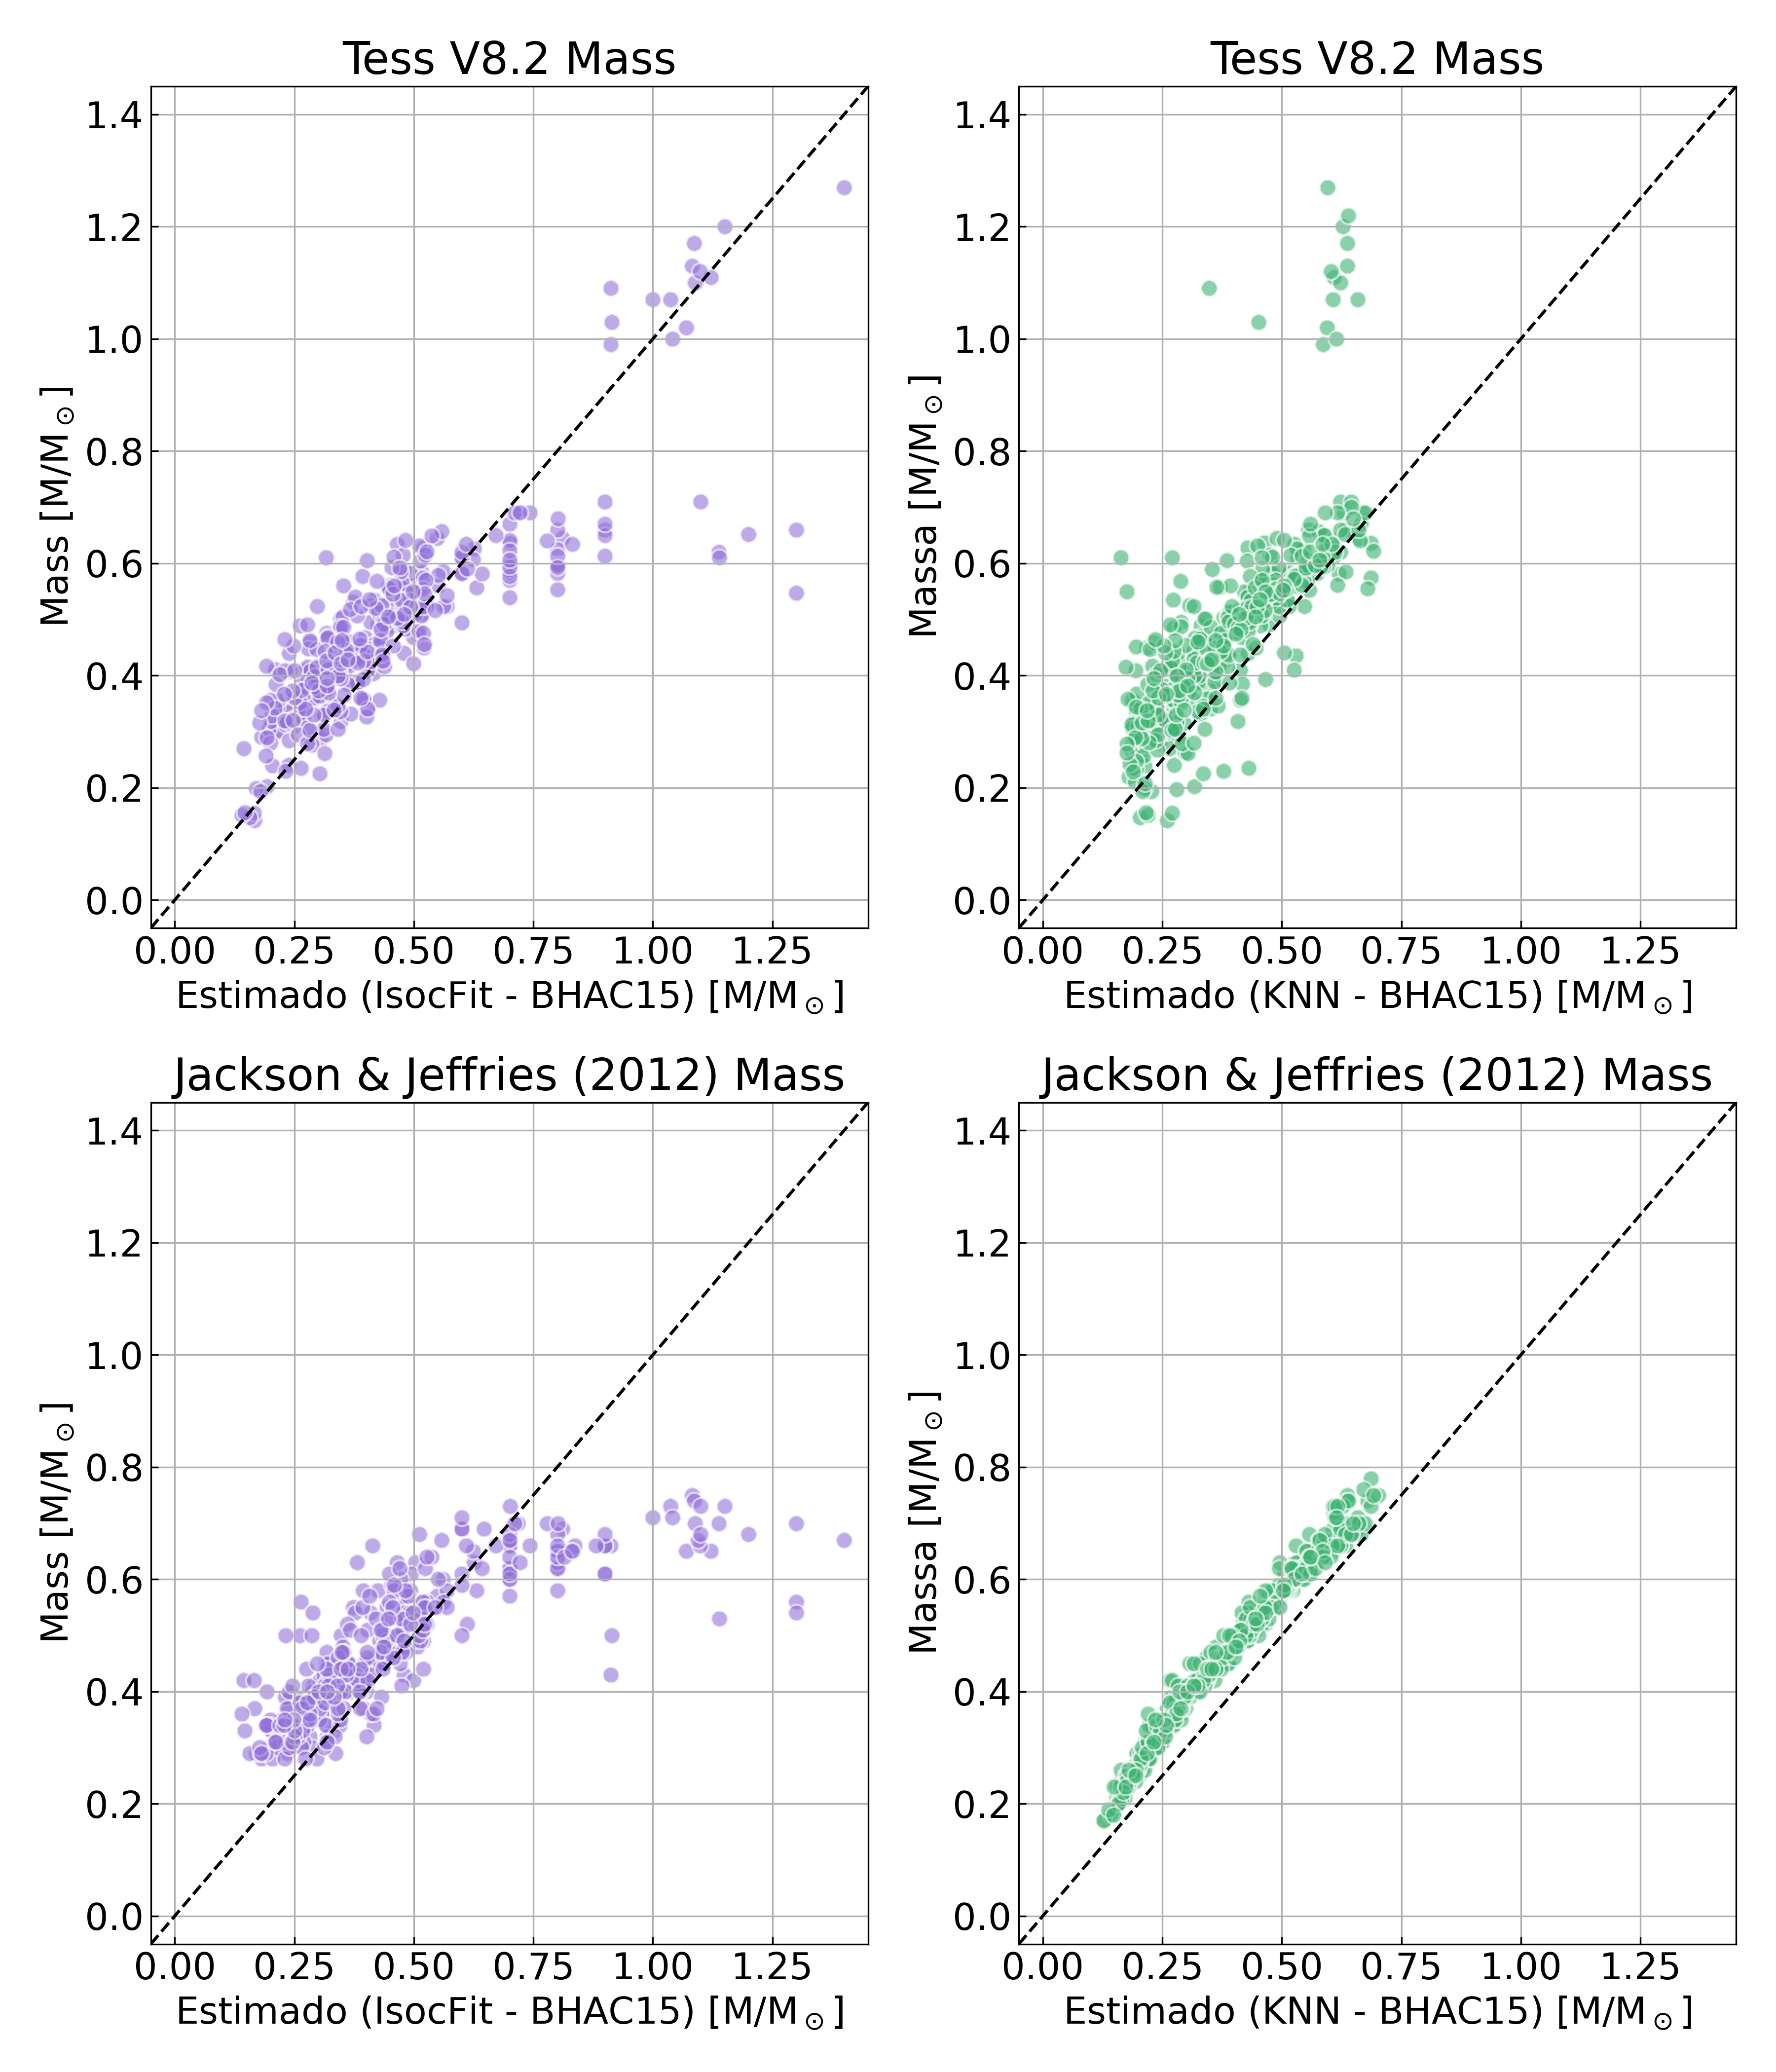
\includegraphics[width=\columnwidth]{figures/ngc2516_results_report.png}
	\caption{Mass estimation performance in NGC 2516 comparing \texttt{IsocFit} (left) and $k$-NN BHAC15 (right) against TESS V8.2 (top) and \citet{jackson2012why} (bottom).}
	\label{fig:ngc2516_results}
\end{figure}

For $M \le 0.7\,M_\odot$, $k$-NN regression demonstrates linear tracking against \citet{jackson2012why} empirical values ($R^2 = 0.97$), validating ML Mass--Magnitude modeling for mature open clusters.


\section{Discussion}
\label{sec:discussion}

Our comparative analysis across five open clusters highlights complementary strengths between 2D Bayesian isochrone fitting and machine-learning Mass--Magnitude relationships:

\begin{enumerate}
    \item **Young PMS Clusters ($t < 10$~Myr):** 2D Bayesian \texttt{IsocFit} is essential when individual stellar ages and posterior standard deviations ($\sigma_M, \sigma_t$) are required to quantify cluster age spreads. However, high differential extinction ($A_V$) and accretion veiling increase HR position scatter.
    \item **Main-Sequence Clusters ($t > 100$~Myr):** As stars settle onto the ZAMS, theoretical tracks merge, causing HR grid minimization degeneracies. Here, $k$-NN machine learning regressors trained on single-band magnitudes (*Gaia* $G$ or $V$) eliminate track-folding ambiguity, yielding superior mass recovery ($R^2 \ge 0.96$).
    \item **Spectroscopic Activity Filtering:** Incorporating Equivalent Widths ($\text{H}\alpha$, $\text{Li}\,\text{I}$) prevents actively accreting CTTS stars ($\text{EW}(\text{H}\alpha) \ge 10\,\text{\AA}$) from skewing photometric $T_{\text{eff}}$ dereddening vectors.
\end{enumerate}


\section{Conclusions}
\label{sec:conclusions}

We have conducted a systematic benchmark of stellar mass, age, and physical parameter estimation techniques across five open clusters spanning $\sim 1\text{--}150$~Myr.

Key conclusions include:
\begin{enumerate}
    \item \texttt{IsocFit} 2D Bayesian estimation incorporating IMF priors provides robust $1\text{-}\sigma$ posterior mass and age distributions for young pre-main-sequence stars.
    \item Machine-learning Mass--Magnitude relationships (RMM) using $k$-NN regressors outperform traditional grid interpolation for stars near the ZAMS ($t \ge 100$~Myr), achieving median mass uncertainties of $2.1\text{--}3.8\%$.
    \item Derivation of bolometric luminosity and radius following \citet{bell2014pre} combined with spectroscopic EW classification enables automated catalog-wide parameter processing.
\end{enumerate}

All algorithms, models, and interactive HTML report generators are publicly available in the \textsc{SPECTRA} software package (\url{https://github.com/matosjp/spectra}).


\section*{Acknowledgements}

The primary development, algorithmic design, and empirical cluster validations were conducted at the Laboratório de Astrofísica Teórica e Observacional (LATO) at the Universidade Estadual de Santa Cruz (UESC). The authors acknowledge institutional support provided by the Universidade Estadual Paulista (UNESP) during final manuscript preparation. MJV and AHC acknowledge partial funding from UESC projects 2023.0003119-74 and 2025.0033125-91.


\section*{Data Availability}

All observational datasets, theoretical model grids, synthetic control tables, and derived cluster parameter catalogs underlying this article are available in the \textsc{SPECTRA} repository at \url{https://github.com/matosjp/spectra}.


%%%%%%%%%%%%%%%%%%%%%%%%%%%%%%%%%%%%%%%%%%%%%%%%%%

%%%%%%%%%%%%%%%%%%%% REFERENCES %%%%%%%%%%%%%%%%%%

\bibliographystyle{mnras}
\bibliography{mnras_references}

%%%%%%%%%%%%%%%%%%%%%%%%%%%%%%%%%%%%%%%%%%%%%%%%%%

\bsp
\label{lastpage}
\end{document}
